\documentclass[a4paper, openany]{memoir}

\usepackage[utf8]{inputenc}
\usepackage[T1]{fontenc} 
\usepackage[english]{babel}

\usepackage{fancyhdr}
\usepackage{float}

\usepackage{amsmath}
\usepackage{amsthm}
\usepackage{amssymb}
\usepackage{enumitem}
\usepackage{multicol}
\usepackage[bookmarksopen=true,bookmarksopenlevel=2]{hyperref}
\usepackage{tikz}
\usepackage{tikz-qtree}
\usepackage{indentfirst}

\usepackage{listings}
\usepackage{xcolor}

\pagestyle{fancy}
\fancyhf{}
\fancyhead[LE]{\leftmark}
\fancyhead[RO]{\rightmark}
\fancyhead[RE, LO]{ADS}
\fancyfoot[LE, RO]{\thepage}
\fancyfoot[RE, LO]{Pete Gautam}

\definecolor{codegreen}{rgb}{0,0.6,0}
\definecolor{codegray}{rgb}{0.5,0.5,0.5}
\definecolor{codepurple}{rgb}{0.58,0,0.82}
\definecolor{backcolour}{rgb}{0.95,0.95,0.92}

\lstdefinestyle{thestyle}{
    backgroundcolor=\color{backcolour},
    basicstyle=\ttfamily\footnotesize,
    keywordstyle=\color{red!80}\bfseries,
    ndkeywordstyle=\color{blue!80}\bfseries,
    identifierstyle=\color{black},
    commentstyle=\color{codegreen},
    stringstyle=\color{codepurple},
    breakatwhitespace=false,
    breaklines=true,
    captionpos=b,
    keepspaces=true,
    numberstyle=\tiny\color{codegray},
    numbers=left,
    numbersep=2pt,
    showspaces=false,
    showstringspaces=false,
    showtabs=false,
    tabsize=2
}
\lstset{style=thestyle}

\lstdefinelanguage{pseudocode}{ 
    keywords={new, return, this, null, if, in, while, else, for, get, set, class, and, or, not, range},
    ndkeywords={int, char, bool, Array, String, Node, Queue, Set, Trie, void, true, false},
    sensitive=true,
    comment=[l]{//},
    morecomment=[s]{/*}{*/},
    morestring=[b]',
    morestring=[b]"
}

\renewcommand{\headrulewidth}{1.5pt}

\tikzset{every tree node/.style={minimum width=2em,draw},
 blank/.style={draw=none},
 edge from parent/.style=
 {draw,edge from parent path={(\tikzparentnode) -- (\tikzchildnode)}},
 level distance=1.5cm,
 black/.style={draw=black},
 }
\usetikzlibrary{backgrounds}
\usetikzlibrary{shapes}

\chapterstyle{thatcher}

\begin{document}
\chapter{Algorithms}

\section{Analysing Algorithms}
An algorithm is a well-defined procedure that is used to solve a problem in a finite period of time, e.g. sorting an array. It can be written in natural language, computer language (pseudocode or an actual language) or hardware design. There are many applications of algorithms, not just in computing!

\noindent Algorithm analysis aims to check the correctness and the running time of the algorithm.

\subsection{Example of an algorithm: Insertion sort}
The algorithm \texttt{insertionSort} is used to sort arrays. The following is a psuedocode for the algorithm:
\begin{lstlisting}[language=pseudocode]
int insertionSort(Array<int> array):
    // loop through the entire array
    for (int j = 1; j < n; j++):
        int key = array[j]
        int i = j-1
        // shift all the elements in the sorted sublist that are 
        // bigger than key
        while (i >= 0 and array[i] > key):
            array[i+1] = array[i]
            i--
        array[i+1] = key
\end{lstlisting}
This algorithm works by increasing the sorted sublist from the left by comparisons. We explain this with an example. Assume that we want to sort the array \texttt{[5, 2, 4, 6, 1]} using insertion sort. At the start, our sorted sublist only consists of the first element \texttt{5}. During the first iteration, we have the following setting for the array:
\begin{center}
    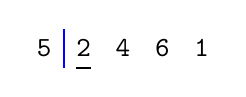
\begin{tikzpicture}
        \node at (.5, .25) {\texttt{5}};
        \draw[thick] (.9, 0) -- (1.1, 0);
        \draw [thick, blue] (.75, 0) -- (.75, .5);
        \node at (1, .25) {\texttt{2}};
        \node at (1.5, .25) {\texttt{4}};
        \node at (2, .25) {\texttt{6}};
        \node at (2.5, .25) {\texttt{1}};
    \end{tikzpicture}
\end{center}
The number \texttt{2} (underlined black) is the \texttt{key}. We want to add it to the sorted sublist (to the left of the blue bar), so we must place it before \texttt{5}.
\begin{center}
    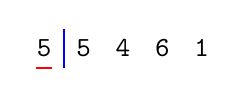
\begin{tikzpicture}
        \node at (.5, .25) {\texttt{5}};
        \draw[thick, red] (.4, 0) -- (.6, 0);
        \draw [thick, blue] (.75, 0) -- (.75, .5);
        \node at (1, .25) {\texttt{5}};
        \node at (1.5, .25) {\texttt{4}};
        \node at (2, .25) {\texttt{6}};
        \node at (2.5, .25) {\texttt{1}};
    \end{tikzpicture}
\end{center}
So, we make the element at the second position \texttt{5}. The location where the \texttt{key} moves is highlighted in red (this is the value of \texttt{i+1}).
\begin{center}
    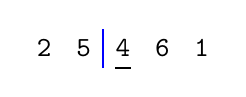
\begin{tikzpicture}
        \node at (.5, .25) {\texttt{2}};
        \draw[thick] (1.4, 0) -- (1.6, 0);
        \draw [thick, blue] (1.25, 0) -- (1.25, .5);
        \node at (1, .25) {\texttt{5}};
        \node at (1.5, .25) {\texttt{4}};
        \node at (2, .25) {\texttt{6}};
        \node at (2.5, .25) {\texttt{1}};
    \end{tikzpicture}
\end{center}
Now, the sorted sublist has 2 elements. We now aim to move the next element \texttt{4} into the sublist- it should be placed between \texttt{2} and \texttt{5}.
\begin{center}
    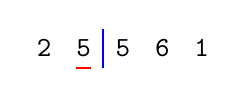
\begin{tikzpicture}
        \node at (.5, .25) {\texttt{2}};
        \draw[thick, red] (.9, 0) -- (1.1, 0);
        \draw [thick, blue] (1.25, 0) -- (1.25, .5);
        \node at (1, .25) {\texttt{5}};
        \node at (1.5, .25) {\texttt{5}};
        \node at (2, .25) {\texttt{6}};
        \node at (2.5, .25) {\texttt{1}};
    \end{tikzpicture}
\end{center}
Because \texttt{4} is to be placed between \texttt{2} and \texttt{5}, we only copy \texttt{5} to the third position; \texttt{2} doesn't get copied to the second position. We now add the element \texttt{4} at the second position.
\begin{center}
    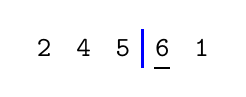
\begin{tikzpicture}
        \node at (.5, .25) {\texttt{2}};
        \draw[thick] (1.9, 0) -- (2.1, 0);
        \draw [thick, blue] (1.75, 0) -- (1.75, .5);
        \node at (1, .25) {\texttt{4}};
        \node at (1.5, .25) {\texttt{5}};
        \node at (2, .25) {\texttt{6}};
        \node at (2.5, .25) {\texttt{1}};
    \end{tikzpicture}
\end{center}
Now, we want to place \texttt{6} within the sorted sublist. It is at the correct position right now.
\begin{center}
    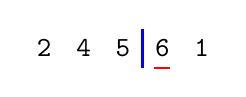
\begin{tikzpicture}
        \node at (.5, .25) {\texttt{2}};
        \draw[thick, red] (1.9, 0) -- (2.1, 0);
        \draw [thick, blue] (1.75, 0) -- (1.75, .5);
        \node at (1, .25) {\texttt{4}};
        \node at (1.5, .25) {\texttt{5}};
        \node at (2, .25) {\texttt{6}};
        \node at (2.5, .25) {\texttt{1}};
    \end{tikzpicture}
\end{center}
Since \texttt{6} is already at the correct position, we have nothing to move- \texttt{6} stays where it is.
\begin{center}
    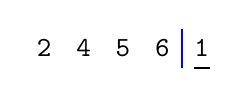
\begin{tikzpicture}
        \node at (.5, .25) {\texttt{2}};
        \draw[thick] (2.4, 0) -- (2.6, 0);
        \draw [thick, blue] (2.25, 0) -- (2.25, .5);
        \node at (1, .25) {\texttt{4}};
        \node at (1.5, .25) {\texttt{5}};
        \node at (2, .25) {\texttt{6}};
        \node at (2.5, .25) {\texttt{1}};
    \end{tikzpicture}
\end{center}
Now, we shall move \texttt{1} to the start of the array.
\begin{center}
    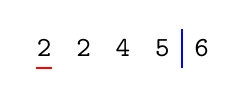
\begin{tikzpicture}
        \node at (.5, .25) {\texttt{2}};
        \draw[thick, red] (.4, 0) -- (.6, 0);
        \draw [thick, blue] (2.25, 0) -- (2.25, .5);
        \node at (1, .25) {\texttt{2}};
        \node at (1.5, .25) {\texttt{4}};
        \node at (2, .25) {\texttt{5}};
        \node at (2.5, .25) {\texttt{6}};
    \end{tikzpicture}
\end{center}
To move \texttt{1} to the start of the array, we shift all the elements within the sorted array one to the right. The element \texttt{1} gets placed at the first position.
\begin{center}
    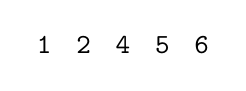
\begin{tikzpicture}
        \node at (.5, .25) {\texttt{1}};
        \node at (1, .25) {\texttt{2}};
        \node at (1.5, .25) {\texttt{4}};
        \node at (2, .25) {\texttt{5}};
        \node at (2.5, .25) {\texttt{6}};
    \end{tikzpicture}
\end{center}
After we place \texttt{1} at the start, there is nothing to the right of the sorted sublist. This means that we have sorted the entire array.

\noindent Insertion sort is a stable sorting algorithm, meaning that the relative order of the elements with the same value are maintained. Also, the sorting algorithm is in-place, meaning that we don't need to create another array in the process.

\subsection{Analysing algorithms}
We can look at the running time to analyse algorithms. We typically focus on the worst case. 

\noindent This can be done using experimental studies- we run the algorithm with a single change (e.g. a larger size of array), and see how that affects the time it takes for the algorithm to run. Such studies are called empirical studies.

\noindent Experimental studies have many limitations. We need to implement the algorithm, and this might be difficult. It is not possible to conclude that the difference we see in the running time for two different inputs comes just from the difference (e.g. the operating system is more busy when running only one of the algorithms). Nevertheless, we consider algorithms run on the same hardware and software as being comparable.

\noindent Instead, we look into theoretical approaches. We don't need to implement the algorithm. Also, it is possible to consider all the input sizes. Moreover, we can evaluate the speed of the algorithm irrespective of the hardware and the software environment.

\subsubsection{Counting Primitive operations}
Primitive operations are basic computations performed in an algorithm. Their implementation is not important because we assume it takes a constant amount of time. Examples of primitive operations include assigning a value, indexing an array, calling a method, etc.

\noindent Consider the following algorithm to compute the element with maximum value in an array, which also highlights the primitive operations:
\begin{lstlisting}[language=pseudocode]
int max(Array<int> array):
    int max = array[0]
    for (int i = 1; i < array.length; i++):
        if array[i] > max:
            max = array[i]
    return max
\end{lstlisting}
In line 2, we have 2 primitive operations- assigning a variable a value, and indexing an array. Similarly, returning a value in line 6 is a primitive operation.

\noindent The for loop in line 3 isn't a primitive operation. This is because it is repeated \texttt{array.length} times. So, line 3 has \texttt{2n} primitive operations for assigning a value and checking whether \texttt{i < array.length}; and \texttt{2(n-1)} for assigning and incrementing \texttt{i}. Here, \texttt{n} is the length of the array. Similarly, any operation within the body of the for loop runs \texttt{n-1} primitive operations (since we're starting for \texttt{1}, not \texttt{0}). The if condition runs \texttt{n-1} times only if we're in the worst case; at the best case, the condition doesn't run once. In total, there are \texttt{8n-3} primitive operations in the worst case; in the best case, there are \texttt{6n-1} primitive operations.

\noindent To estimate the running time based on the primitive operations, we define the function $T$ that is the running time of the worst-case of the algorithm. Then, $a(8n - 3) \leq T(n) \leq b(8n-3)$. So, $T(n)$ is bounded by two linear functions.

\noindent When we change the hardware and the software environment, the function $T$ is only affected by a constant factor- the function will still be linear. That is, the algorithm will always have a linear growth rate.

\noindent The growth rate of the running time of an algorithm isn't affected by constant factors and lower-degree terms.

\subsection{Big-Oh Notation}
If we have functions $f$ and $g$, then we say that $f$ is $O(g)$ if there are constants $c$ and $n_0$ such that $f(n) \leq cg(n)$ for $n \geq n_0$. That is, the big-oh notation gives us an upper bound up to a constant factor. 

\noindent If $f = O(g)$, then $g$ grows more than $f$ or $f$ and $g$ have the same growth rate- it isn't possible for $f$ to grow more than $g$. On the other hand, if $g = O(f)$, then $f$ grows more than $g$ or $f$ and $g$ have the same growth rate.

\noindent The Big-Oh notation allows us to perform asymptotic algorithm analysis. That is, we are comparing the algorithm with respect to the input size- it is evaluating the scalability of an algorithm. It is used to judge the asymptotic efficiency of an algorithm. In particular, the Big-Oh notion is used to express asymptotic upper bounds.

\noindent When we have a function $f$, the following are the rules for Big-Oh:
\begin{itemize}
    \item If $f$ is of degree $d$, then $f = O(n^d)$- we can drop lower order terms and any constant factors.
    \item If $f = O(n)$ and $f = O(n^2)$, we just say $f = O(n)$ because we want the tightest bound to the function.
    \item If $f = O(3n+5)$, we write $f = O(n)$- we drop lower order terms and constant factors.
\end{itemize}

\noindent Now, assume we want to show that $2n + 10$ is $O(n)$. First, define the functions $f(n) = 2n + 10, g(n) = n$. We now need to find constants $c$ and $n_0$ such that $f(n) \leq cg(n)$ for $n \geq n_0$. We can substitute and simplify as follows:
\[2n + 10 \leq cn \iff (c - 2)n \geq 10 \iff n \geq \frac{10}{c-2}.\]
So, we can set $c = 3$ and $n_0 = 10$.

\noindent Now, let's say we want to show that $7n - 2$ is $O(n)$. So, we have functions $f(n) = 7n - 2, g(n) = n$. Also, define constants $c$ and $n_0$ such that $f(n) \leq cg(n)$ for $n \geq n_0$. Substituting, we get
\[7n - 2 \leq cn \iff (c-7)n \geq -2 \iff n \geq \frac{-2}{c - 7}.\]
So, we can set $c = 8$ and $n_0 = 1$.

\noindent We can also try to show that $n^2$ is not $O(n)$. We do the calculations like above- set $f(n) = n^2$ and $g(n) = n$. Then, let $c$ and $n_0$ be such that for $n \geq n_0 > 0$,
\[n^2 \leq cn \iff n \leq c.\]
But, we should be able choose $n \geq n_0$, which at some point will cross $c$, so $n^2$ is not $O(n)$.

\noindent We now try to show that $3n^3 + 20n^2 + 5$ is $O(n^3)$. So, let $f(n) = 3n^3 + 20n^2 + 5$ and $g(n) = n^3$, and define constants $c$ and $n_0$ such that $f(n) \leq cg(n)$ for $n \geq n_0$. Substituting, we get
\[3n^3 + 20n^2 + 5 \leq cn^3 \iff n^3(c - 3) \geq 20n^2 + 5 \iff n^3 \geq \frac{20n^2 + 5}{c - 3}.\]
So, we can set $c = 4$ and $n_0 = 3$.

\noindent Finally, we want to show that $3 \log n + 5$ is $O(\log n)$. So, let $f(n) = 3 \log n + 5$ and $g(n) = \log n$, and define constants $c$ and $n_0$ such that $f(n) \leq cg(n)$ for $n \geq n_0$. Substituting, we get
\[3\log n + 5 \leq c\log n \iff (c - 3) \log n \geq 5 \iff \log n \geq \frac{5}{c - 3}.\]
So, we can set $c = 4$ and $n_0 = 2^5 = 32$.

\noindent We now look at another Big-Oh rule: 
\begin{itemize}
    \item If $T_1 = O(f)$ and $T_2 = O(g)$, then $T_1 + T_2 = O(\max(f, g))$.
    \item If $T_1 = O(f)$ and $T_2 = O(g)$, then $T_1 T_2 = O(fg)$.
    \item If $T(n) = (\log n)^k$, then $T(n) = O(n)$ for all $k$.
\end{itemize}

\subsubsection{Computing Running Time}
There are many rules when we compute the running time. These are:
\begin{itemize}
    \item If we have a loop, then the running time is the running time of the body of the loop multiplied by the number of times the loop is repeated.
    \item In particular, if we have nested loops, then the running time gets multiplied. For example, the running time of the function below is $O(n^3)$ since there are $3$ loops of length $n$:
\begin{lstlisting}[language=pseudocode]
void algorithm(int n):
    int x = 0;
    for (int i = 0; i < n; i++):
        for (int j = 0; j < n; j++):
            for (int k = 0; k < n; k++):
                x++;
\end{lstlisting}
    \item If we have consecutive statements, we just take the maximum since it is additive.
    \item If we have many if-then-else clauses, we take the branch with the highest running branch.
\end{itemize}
We revisit the insertion sort now. Below is the psuedocode which highlights the number of operations per line.
\begin{lstlisting}[language=pseudocode]
int insertionSort(Array<int> array):
    // 2n + 2(n-1) operations
    for (int j = 1; j < n; j++):
        // 2(n-1) operations
        int key = array[j]
        // n-1 operations
        int i = j-1
        // (max) n(n+1) operations
        while (i >= 0 and array[i] > key):
            // (max) n(n+1)-1 operations
            array[i+1] = array[i]
            // (max) n(n+1)-1 operations
            i--
        // n-1 operations
        array[i+1] = key
\end{lstlisting}
In the best case, we never enter the while loop- the array is already sorted. The running time is $O(n)$. On the other hand, the \texttt{while} loop runs from \texttt{i=j-1} to \texttt{i=0} each iteration in the worst case, so in total it runs 
\[1 + 2 + 3 + \cdots + n = \frac{1}{2} n(n+1)\]
times. So, the running time is $O(n^2)$.

\subsubsection{Common growth rates}
The following are common growth rates:
\begin{itemize}
    \item $O(1)$ or constant;
    \item $O(\log n)$ or logarithmic;
    \item $O(\sqrt{n})$ or fractional power;
    \item $O(n)$ or linear;
    \item $O(n \log n)$ or quasilinear;
    \item $O(n^2)$ or quadratic;
    \item $O(n^3)$ or cubic.
\end{itemize}
They are listed in order of runtime with respect to growth rate- $O(1)$ is the fastest, while $O(n^3)$ is the slowest (in this array). 

\noindent If we want to show that $\sqrt{n}$ lies between $\log n$ and $n$, we can show $\sqrt{n} = O(n)$ and $\log n = O(\sqrt{n})$. Taking $c = 1$ and $n_0 = 4$, we have $\sqrt{n} \leq cn$, while taking $c = 1$ and $n_0 = 8$, we have $\log n \leq c \sqrt{n}$.

\noindent Further complexities $O(2^n)$ (exponential) and $O(n!)$ (factorial) are possible, but are exceptionally slow in practice.

\noindent We now consider the running time of few algorithms. First, consider the following psuedocode
\begin{lstlisting}[language=pseudocode]
// computes the sum of the squares between 0 and n
int squaresSum(int n):
    int i = 0 // O(1)
    int sum = 0 // O(1)
    while (i < n): // O(n)
        i++ // O(n)
        sum += i*i // O(n)
    return sum // O(1)
\end{lstlisting}
The highest operation here is $O(n)$, so the function is $O(n)$. The following algorithm also performs the same computation, but using a formula
\begin{lstlisting}[language=pseudocode]
// computes the sum of the squares between 0 and n
int squaresSum(int n):
    int sum = n*(n+1)*(2n+1)/6 // O(1)
    return sum // O(1)
\end{lstlisting}
This function is $O(1)$. So, this function is intrinsically faster than the previous function.
\noindent Now, consider the following function.
\begin{lstlisting}[language=pseudocode]
// computes the integer part of the square root of n
int integerPart(int n):
    int i = 0 // O(1)
    while ((i+1)*(i+1) <= n): // O(sqrt(n))
        i++ // O(sqrt(n))
    return i // O(1)
\end{lstlisting}
We can find that the while loop is $O(\sqrt{n})$ by considering the number of iterations it takes for some integer $n$. For example, if $n = 13$, the loop runs 3 times (when the expression \texttt{(i+1)*(i+1)} equals $1$, $4$ and $9$). Moreover, at the worst case, the loop runs $\sqrt{n}$. Since that is the highest operation here, the function is $O(\sqrt{n})$.

\noindent Now, consider the following algorithms:
\begin{lstlisting}[language=pseudocode]
void algorithm1(int n):
    int sum = 0 // O(1)
    for (i = 0; i < n; i++): // O(n)
        for (j = 0; j < i; j++): // O(n^2)
            sum++
\end{lstlisting}
Here, the inside loop runs for
\[1 + 2 + 3 + \cdots + n = \frac{1}{2}n(n+1) = O(n^2)\]
times. So, the running time of the algorithm is $O(n^2)$.

\noindent The next algorithm to consider is:
\begin{lstlisting}[language=pseudocode]
void algorithm2(int n):
    int sum = 0 // O(1)
    for (int i = 0; i < n; i++): // O(n)
        for (j = 0; j < i*i; j++): // O(n^3)
            for (k = 0; k < j; k++): // O(n^5)
                sum++
\end{lstlisting}
Here, the loop in line 3 runs $n$ times; the loop in line 4 runs at most $n^2$ times for some \texttt{i}; while the loop in line 5 runs at most $n^2$ times for some \texttt{j}- multiplying, we find that the algorithm has runtime $O(n^5)$.

\noindent We now consider the final algorithm below:
\begin{lstlisting}[language=pseudocode]
void algorithm3(int n):
    int sum = 0 // O(1)
    for (int i = 1; i <= n; i++): // O(n)
        for (int j = 1; j <= i*i; j++): // O(n^3)
            if (j % i == 0): // O(n^3)
                for (int k = 1; k <= j; k++): // O(n^4)
                    sum++ // O(n^4)
\end{lstlisting}
The \texttt{if} condition is only true if \texttt{j} is \texttt{i}, \texttt{2i}, and so on up to \texttt{i*i}- this loop runs \texttt{i} times with respect to \texttt{j}. So, this algorithm has runtime $O(n^4)$.

\subsubsection{More asymptotic notations}
Now, we define more asymptotic notations:
\begin{itemize}
    \item $f = \Omega(g)$ if there are constants $c$ and $n_0$ such that $f(n) \geq cg(n)$ for $n \geq n_0$, i.e. $f$ is bounded below by a factor of $g$.
    \item $f = \Theta(g)$ if and only if $f = O(g)$ and $f = \Omega(g)$, i.e. the functions grow at the same rate.
\end{itemize}
For example, let $f(n) = 5n^3 + 2$. Then, $f = O(n^3)$ (using $c = 6, n_0 = 2$), but also $f = O(n^4)$ or any bigger power. Similarly, $f = \Omega(n^3)$ (using $c = 4, n_0 = 0$) and $f = \Omega(n^2)$ or any smaller power. But, $f = \Theta(n^3)$ only, and not any other power- this is a tight bound.
\newpage

\section{Recursive Algorithms}
A function is recursive if it is refers to itself from within the function. An example of this is the factorial function:
\begin{lstlisting}[language=pseudocode]
// returns the factorial of the number n
int factorial(int n):
    // base case
    if (n == 0):
        return 1
    // recursive case
    return n * factorial(n-1)
\end{lstlisting}
A recursive algorithm calls itself, but with different parameter(s) so that we get closer to the base case. Therefore, a recursive algorithm must have a base case for the algorithm to terminate.

\noindent One way to study a recursive algorithm is using a recursion trace. An example of the recursion trace for the \texttt{factorial} function is shown below with \texttt{n = 4}:
\begin{center}
    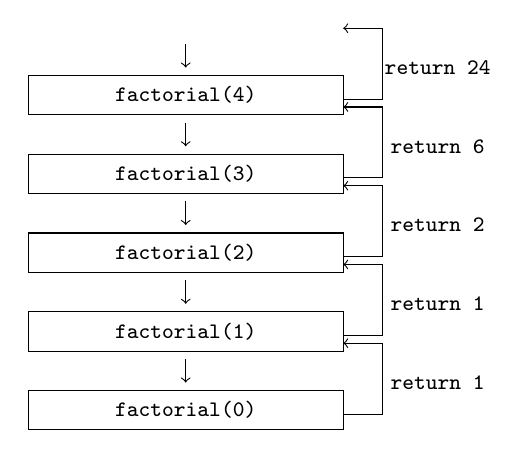
\begin{tikzpicture}
        \foreach \x in {0, 1, 2, 3, 4} {
            \draw (-2, \x) -- (-2, \x + 0.5) -- (2, \x + 0.5) -- (2, \x) -- cycle;
            \draw[->] (0, \x + 0.9) -- (0, \x + 0.6);
            \draw (2, \x + 0.2) -- (2.5, \x + 0.2) -- (2.5, \x + 1.1) -- (2, \x + 1.1)[->];
            \node at (0, \x + 0.25) {\footnotesize\texttt{factorial(\x)}};
        }
        \node at (3.2, 0.6) {\footnotesize\texttt{return 1}};
        \node at (3.2, 1.6) {\footnotesize\texttt{return 1}};
        \node at (3.2, 2.6) {\footnotesize\texttt{return 2}};
        \node at (3.2, 3.6) {\footnotesize\texttt{return 6}};
        \node at (3.2, 4.6) {\footnotesize\texttt{return 24}};
    \end{tikzpicture}
\end{center}
Therefore, the final output is \texttt{24}.

\subsection{Linear Recursion}
A linear recursion makes at most one recursive call per invocation. The amount of space needed to track the nested calls grows linearly. Such functions are linear because it grows at the same rate as the input, e.g. the recursion trace grows one every time we increase the input.

\noindent Another example of a linear recursion is the sum of the values within an array.
\begin{lstlisting}[language=pseudocode]
// returns the sum of the array
int listSum(Array<int> array):
    // base case
    if (array.length == 0):
        return 0
    // recursive case
    return array[0] + listSum(array[1:])
\end{lstlisting}
This function is a terminating recursive function since there is a base case and the \texttt{array} always gets smaller. We now look at the recursive trace with \texttt{array = [1, 3, 8]}:
\begin{center}
    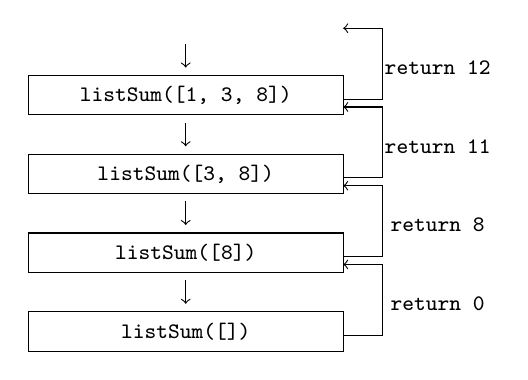
\begin{tikzpicture}
        \foreach \x in {0, 1, 2, 3} {
            \draw (-2, \x) -- (-2, \x + 0.5) -- (2, \x + 0.5) -- (2, \x) -- cycle;
            \draw[->] (0, \x + 0.9) -- (0, \x + 0.6);
            \draw (2, \x + 0.2) -- (2.5, \x + 0.2) -- (2.5, \x + 1.1) -- (2, \x + 1.1)[->];
        }
        \node at (0, 0.25) {\footnotesize\texttt{listSum([])}};
        \node at (0, 1.25) {\footnotesize\texttt{listSum([8])}};
        \node at (0, 2.25) {\footnotesize\texttt{listSum([3, 8])}};
        \node at (0, 3.25) {\footnotesize\texttt{listSum([1, 3, 8])}};
        
        \node at (3.2, 0.6) {\footnotesize\texttt{return 0}};
        \node at (3.2, 1.6) {\footnotesize\texttt{return 8}};
        \node at (3.2, 2.6) {\footnotesize\texttt{return 11}};
        \node at (3.2, 3.6) {\footnotesize\texttt{return 12}};
    \end{tikzpicture}
\end{center}
The output, in this case, is \texttt{12}. Moreover, both the functions \texttt{factorial} and \texttt{listSum} are $O(n)$.

\subsection{Tail Recursion}
Recursion is very useful in designing short and intuitive algorithms. But, in practice, it has a cost of memory per recursive call- we keep track of all the calls in the recursive trace by a stack. We can always make a non-recursive algorithm for a recursive one if this is a big issue. 

\noindent However, sometimes we can be more efficient by just using \texttt{tail recursion}. In tail recursion, the recursion is linear and the last operation in the algorithm. An example of tail recursion is the following algorithm:
\begin{lstlisting}[language=pseudocode]
// reverses an array
void reverse(Array<int> array, int i, int j):
    if (i < j):
        array[i], array[j] = array[j], array[i]
        reverse(array, i+1, j-1)
\end{lstlisting}
We start the algorithm with \texttt{reverse(array, 0, array.length-1)}. This is tail recursive since the final line is the only place where we find the recursive call, and the call is linear since there is only one call. The function \texttt{reverse} was also tail recursive for the same reason. However, the function \texttt{factorial} was not tail recursive since it ended with \texttt{return n * factorial(n-1)}- we perform an operation on the value. We can rewrite the function as shown below to make it tail recursive.
\begin{lstlisting}[language=pseudocode]
int factorial(int n, int acc):
    if (n == 0):
        return acc
    return factorial(n-1, n * acc)
\end{lstlisting}
We can also write this algorithm as an iterative algorithm:
\begin{lstlisting}[language=pseudocode]
int factorial(int n, int acc):
    int i = n
    int factorial = 1
    while (i > 0):
        factorial *= i
        i--
    return factorial
\end{lstlisting}

\subsection{Binary recursion}
A binary operation makes two recursive calls. An example of this is computing the fibonacci number:
\begin{lstlisting}[language=pseudocode]
int fib(int n):
    // base cases (n = 1 or n = 0)
    if n <= 1:
        return n
    // binary recursion case
    return fib(n-1) + fib(n-2)
\end{lstlisting}
The algorithm is very inefficient. This has a recursion tree shown below for \texttt{n = 5}.
\begin{center}
    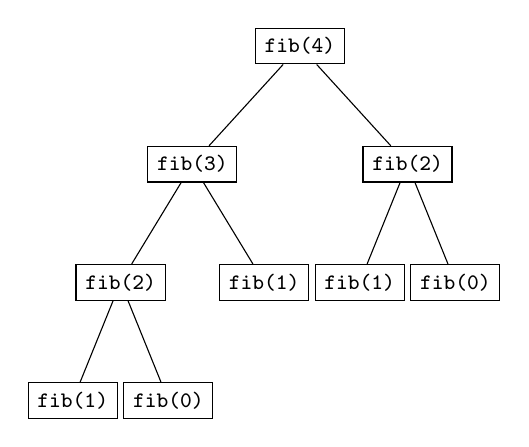
\begin{tikzpicture}
        \Tree
        [.\footnotesize\texttt{fib(4)}
            [.\footnotesize\texttt{fib(3)}
                [.\footnotesize\texttt{fib(2)}
                    [.\footnotesize\texttt{fib(1)}
                    ]
                    [.\footnotesize\texttt{fib(0)}
                    ]
                ]
                [.\footnotesize\texttt{fib(1)}
                ]
            ]
            [.\footnotesize\texttt{fib(2)}
                [.\footnotesize\texttt{fib(1)}
                ]
                [.\footnotesize\texttt{fib(0)}
                ]
            ]
        ]
    \end{tikzpicture}
\end{center}
This implementation is very inefficient since there are a lot of duplicates. For example, the right branch of \texttt{fib(4)} is also the left branch of \texttt{fib(3)}. Since the recursion tree grows twice with respect to input size, the running time of this function is $O(2^n)$.

\subsection{Analysing Recursive Algorithms}
The running time $T(n)$ of a recursive algorithm can be described by a recurrence equation. For example, consider the factorial function below
\begin{lstlisting}[language=pseudocode]
int factorial(int n):
    // T(0) = O(1)
    if (n == 0):
        return 1
    // T(n) = T(n-1) + O(1)
    return n * factorial(n-1)
\end{lstlisting}
So, the base case has running time $T(0) = O(1)$- it is $T(0)$ since the base case applies when \texttt{n=0}. On the other hand, the recursive case has running time $T(n) = T(n-1) + O(1)$. This is annotated in the pseudocode above.

\noindent We can solve the recursive equation iteratively. We find that
\begin{align*}
    T(n) &= T(n-1) + O(1) \\
    &= (T(n-2) + O(1)) + O(1) \\
    &= T(n-2) + 2O(1) \\
    &= T(n-3) + 3O(1) \\
    &= \cdots \\
    &= T(0) + nO(1) \\
    &= (n+1)O(1).
\end{align*}
Therefore, $T$ is $O(n)$. 

\noindent Another way of computing the running time is using recursion tree. We draw until the base case and then use its running time and add the running time for each level, and then multiplying it by the height of the tree.

\noindent Finally, we can apply the Master theorem to compute the running time. This is a generalisation of recursive tree. It states that if the recurrence is
\[T(n) = aT(n/b) + f(n)\]
where $a \geq 1, b \geq 1$, we have one of the three cases:
\begin{itemize}
    \item If $f = \Theta(n^c)$, where $c < \log_b a$, then $T(n) = \Theta(n^{\log_b a})$;
    \item If $f = \Theta(n^c)$, where $c = \log_b a$, then $T(n) = \Theta(n^c \log n)$;
    \item If $f = \Theta(n^c)$, where $c > \log_b a$, then $T(n) = \Theta(f)$.
\end{itemize}
\newpage

\section{Sorting Algorithms}
There are many possible approaches in finding a sorting algorithm. For example, insertion sort takes an incremental approach- we assume that a sublist is sorted, and we expand that sublist one at a time. This is not the most optimal approach since it is of order $O(n^2)$.

\subsection{Selection Sort}
Selection sort is another incremental approach that aims to expand the sublist by adding the smallest element to the sorted sublist from the unsorted subsection by performing swaps. It has the following pseudocode:
\begin{lstlisting}[language=pseudocode]
void selectionSort(Array<int> array):
    for (int i = 0; i < n-1; i++):
        // compute the index of the minimum element in the  
        // unsorted sublist
        int min = i
        for (int j = i; j < n; j++):
            if (array[j] < array[min]):
                min = j
        // swap the element in this index with the minimum element
        array[i], array[min] = array[min], array[i]
\end{lstlisting}
We now visualise how the algorithm works using the array \texttt{[2, 5, 3, 1, 4, 7]}. The initial state of the array, after entering the loop, is:
\begin{center}
    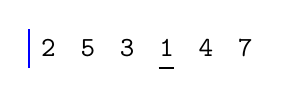
\begin{tikzpicture}
        \draw [thick, blue] (.25, 0) -- (.25, .5);
        \draw[thick] (1.9, 0) -- (2.1, 0);
        \node at (.5, .25) {\texttt{2}};
        \node at (1, .25) {\texttt{5}};
        \node at (1.5, .25) {\texttt{3}};
        \node at (2, .25) {\texttt{1}};
        \node at (2.5, .25) {\texttt{4}};
        \node at (3, .25) {\texttt{7}};
    \end{tikzpicture}
\end{center}
The blue wall represents the sorted sublist- with every iteration, it increases by 1. At the start, there is no element in this sublist. We now add the smallest element \texttt{1} into the first index by swapping it with the element just after the blue wall.
\begin{center}
    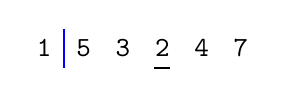
\begin{tikzpicture}
        \draw [thick, blue] (.75, 0) -- (.75, .5);
        \draw[thick] (1.9, 0) -- (2.1, 0);
        \node at (.5, .25) {\texttt{1}};
        \node at (1, .25) {\texttt{5}};
        \node at (1.5, .25) {\texttt{3}};
        \node at (2, .25) {\texttt{2}};
        \node at (2.5, .25) {\texttt{4}};
        \node at (3, .25) {\texttt{7}};
    \end{tikzpicture}
\end{center}
Now, we swap the smallest element \texttt{2} with the element after the wall \texttt{5}.
\begin{center}
    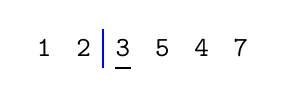
\begin{tikzpicture}
        \draw [thick, blue] (1.25, 0) -- (1.25, .5);
        \draw[thick] (1.4, 0) -- (1.6, 0);
        \node at (.5, .25) {\texttt{1}};
        \node at (1, .25) {\texttt{2}};
        \node at (1.5, .25) {\texttt{3}};
        \node at (2, .25) {\texttt{5}};
        \node at (2.5, .25) {\texttt{4}};
        \node at (3, .25) {\texttt{7}};
    \end{tikzpicture}
\end{center}
Here, the smallest element is the element just after the blue wall- we perform no swaps.
\begin{center}
    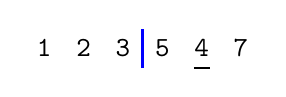
\begin{tikzpicture}
        \draw [thick, blue] (1.75, 0) -- (1.75, .5);
        \draw[thick] (2.4, 0) -- (2.6, 0);
        \node at (.5, .25) {\texttt{1}};
        \node at (1, .25) {\texttt{2}};
        \node at (1.5, .25) {\texttt{3}};
        \node at (2, .25) {\texttt{5}};
        \node at (2.5, .25) {\texttt{4}};
        \node at (3, .25) {\texttt{7}};
    \end{tikzpicture}
\end{center}
Then, we swap the elements \texttt{5} and \texttt{4}.
\begin{center}
    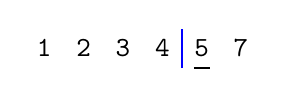
\begin{tikzpicture}
        \draw [thick, blue] (2.25, 0) -- (2.25, .5);
        \draw[thick] (2.4, 0) -- (2.6, 0);
        \node at (.5, .25) {\texttt{1}};
        \node at (1, .25) {\texttt{2}};
        \node at (1.5, .25) {\texttt{3}};
        \node at (2, .25) {\texttt{4}};
        \node at (2.5, .25) {\texttt{5}};
        \node at (3, .25) {\texttt{7}};
    \end{tikzpicture}
\end{center}
Here also, we make no swaps since \texttt{5} is the smallest element in the unsorted sublist. Then, we end up at the last element in the array- this element must have been bigger than all the elements before it. Therefore, we have sorted the array. The sorted array is
\begin{center}
    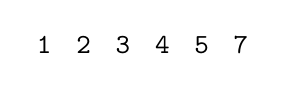
\begin{tikzpicture}
        \node at (.5, .25) {\texttt{1}};
        \node at (1, .25) {\texttt{2}};
        \node at (1.5, .25) {\texttt{3}};
        \node at (2, .25) {\texttt{4}};
        \node at (2.5, .25) {\texttt{5}};
        \node at (3, .25) {\texttt{7}};
    \end{tikzpicture}
\end{center}
In the pseudocode, the maximum number of iterations with respect to \texttt{i} is \texttt{n-1}, while the maximum number of iterations with respect to \texttt{j} is \texttt{n-1}. So, the running time of selection sort is $O(n^2)$.

\subsection{Merge sort}
We now look at divide-and-conquer approaches of sorting. This is typically a recursive algorithm and has a better running time than an incremental approach. First, we divide a problem into smaller subproblems; solve the subproblems recursive, until we get to the base case; and combine the solutions to form the solution to the bigger problem. Such algorithms are more efficient than incremental algorithms. Examples of this approach are merge and quick sort.

\noindent Merge sort is a divide-and-conquer algorithm, so we first divide the input into subarrays of half the length; sort the subarrays recursively using merge sort; and finally combine the merged subarrays to sort the entire array. 

\noindent The combination process, called \texttt{merge} is given below:
\begin{lstlisting}[language=pseudocode]
// array[p:q] is the left subarray, while array[q:r] is the right
// subarray. Both subarrays are sorted.
void merge(Array<int> array, int p, int q, int r):
    Array<int> left = array[p:q]
    Array<int> right = array[q+1:r]
    left.add(Integer.MAX_VALUE)
    right.add(Integer.MAX_VALUE)
    int i = 0
    int j = 0
    for (int k = p; k <= r; k++):
        // if the left elt is smaller, add that
        if (left[i] <= right[j]):
            array[k] = left[i]
            i++
        // otherwise, add the elt from the right
        else:
            array[k] = right[j]
            j++
\end{lstlisting}
Using \texttt{Integer.MAX\_VALUE}, we can avoid extra conditions to check when the two arrays have been scanned. We show how this function works by considering how it merges the array \texttt{[1, 3, 4, 2, 5, 6]} with \texttt{p=0}, \texttt{q=2} and \texttt{r=5}:
\begin{center}
    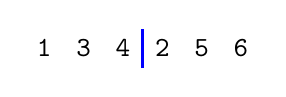
\begin{tikzpicture}
        \draw [thick, blue] (1.75, 0) -- (1.75, .5);
        \node at (.5, .25) {\texttt{1}};
        \node at (1, .25) {\texttt{3}};
        \node at (1.5, .25) {\texttt{4}};
        \node at (2, .25) {\texttt{2}};
        \node at (2.5, .25) {\texttt{5}};
        \node at (3, .25) {\texttt{6}};
    \end{tikzpicture}
\end{center}
By the definition of \texttt{p}, \texttt{q} and \texttt{r}, we can divide the array into 2 left and right sublists, both of which are sorted. We make a copy of these arrays, and enter the while loop:
\begin{center}
    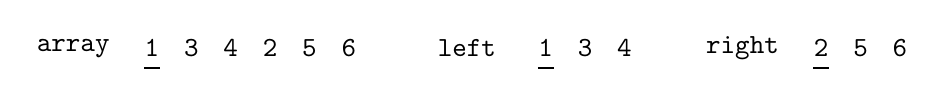
\begin{tikzpicture}
        \draw [thick] (0.4, 0) -- (0.6, 0);
        \node at (-.5, .25) {\texttt{array}};
        \node at (.5, .25) {\texttt{1}};
        \node at (1, .25) {\texttt{3}};
        \node at (1.5, .25) {\texttt{4}};
        \node at (2, .25) {\texttt{2}};
        \node at (2.5, .25) {\texttt{5}};
        \node at (3, .25) {\texttt{6}};

        \draw[thick] (5.4, 0) -- (5.6, 0);
        \node at (4.5, .25) {\texttt{left}};
        \node at (5.5, .25) {\texttt{1}};
        \node at (6, .25) {\texttt{3}};
        \node at (6.5, .25) {\texttt{4}};

        \draw[thick] (8.9, 0) -- (9.1, 0);
        \node at (8, .25) {\texttt{right}};
        \node at (9, .25) {\texttt{2}};
        \node at (9.5, .25) {\texttt{5}};
        \node at (10, .25) {\texttt{6}};         
    \end{tikzpicture}
\end{center}
The variable \texttt{k} keeps track of the indices within the array; the variable \texttt{i} keeps track of the indices within the left sublist; and the variable \texttt{j} keeps track of the indices within the right sublist. Since the highlighted element in the left sublist \texttt{1} is smaller than \texttt{2}, we place \texttt{1} in the first position of the array. We then increment \texttt{k} and \texttt{i}.
\begin{center}
    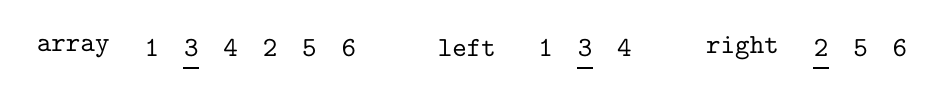
\begin{tikzpicture}
        \draw [thick] (0.9, 0) -- (1.1, 0);
        \node at (-.5, .25) {\texttt{array}};
        \node at (.5, .25) {\texttt{1}};
        \node at (1, .25) {\texttt{3}};
        \node at (1.5, .25) {\texttt{4}};
        \node at (2, .25) {\texttt{2}};
        \node at (2.5, .25) {\texttt{5}};
        \node at (3, .25) {\texttt{6}};

        \draw[thick] (5.9, 0) -- (6.1, 0);
        \node at (4.5, .25) {\texttt{left}};
        \node at (5.5, .25) {\texttt{1}};
        \node at (6, .25) {\texttt{3}};
        \node at (6.5, .25) {\texttt{4}};

        \draw[thick] (8.9, 0) -- (9.1, 0);
        \node at (8, .25) {\texttt{right}};
        \node at (9, .25) {\texttt{2}};
        \node at (9.5, .25) {\texttt{5}};
        \node at (10, .25) {\texttt{6}};         
    \end{tikzpicture}
\end{center}
Now, since \texttt{2} is smaller than \texttt{3}, we add the element from the second array into the array. This time, we increment \texttt{k} and \texttt{j}.
\begin{center}
    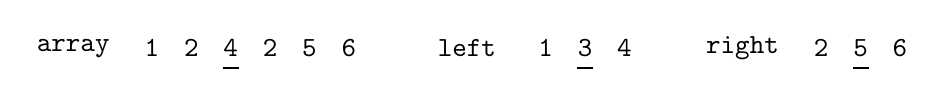
\begin{tikzpicture}
        \draw [thick] (1.4, 0) -- (1.6, 0);
        \node at (-.5, .25) {\texttt{array}};
        \node at (.5, .25) {\texttt{1}};
        \node at (1, .25) {\texttt{2}};
        \node at (1.5, .25) {\texttt{4}};
        \node at (2, .25) {\texttt{2}};
        \node at (2.5, .25) {\texttt{5}};
        \node at (3, .25) {\texttt{6}};

        \draw[thick] (5.9, 0) -- (6.1, 0);
        \node at (4.5, .25) {\texttt{left}};
        \node at (5.5, .25) {\texttt{1}};
        \node at (6, .25) {\texttt{3}};
        \node at (6.5, .25) {\texttt{4}};

        \draw[thick] (9.4, 0) -- (9.6, 0);
        \node at (8, .25) {\texttt{right}};
        \node at (9, .25) {\texttt{2}};
        \node at (9.5, .25) {\texttt{5}};
        \node at (10, .25) {\texttt{6}};         
    \end{tikzpicture}
\end{center}
Since \texttt{3} is smaller than \texttt{5}, we now add \texttt{3} into the array.
\begin{center}
    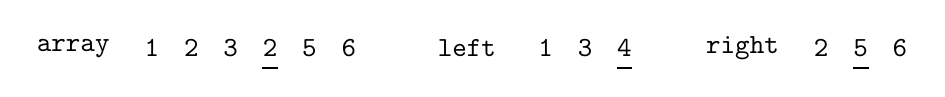
\begin{tikzpicture}
        \draw [thick] (1.9, 0) -- (2.1, 0);
        \node at (-.5, .25) {\texttt{array}};
        \node at (.5, .25) {\texttt{1}};
        \node at (1, .25) {\texttt{2}};
        \node at (1.5, .25) {\texttt{3}};
        \node at (2, .25) {\texttt{2}};
        \node at (2.5, .25) {\texttt{5}};
        \node at (3, .25) {\texttt{6}};

        \draw[thick] (6.4, 0) -- (6.6, 0);
        \node at (4.5, .25) {\texttt{left}};
        \node at (5.5, .25) {\texttt{1}};
        \node at (6, .25) {\texttt{3}};
        \node at (6.5, .25) {\texttt{4}};

        \draw[thick] (9.4, 0) -- (9.6, 0);
        \node at (8, .25) {\texttt{right}};
        \node at (9, .25) {\texttt{2}};
        \node at (9.5, .25) {\texttt{5}};
        \node at (10, .25) {\texttt{6}};         
    \end{tikzpicture}
\end{center}
Still, the element \texttt{4} in the left sublist is smaller than the one in the right sublist, we add \texttt{4} into the array.
\begin{center}
    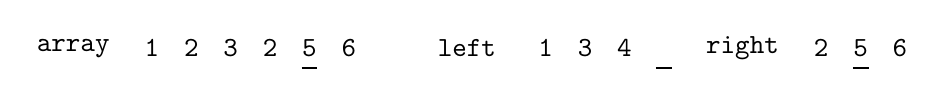
\begin{tikzpicture}
        \draw [thick] (2.4, 0) -- (2.6, 0);
        \node at (-.5, .25) {\texttt{array}};
        \node at (.5, .25) {\texttt{1}};
        \node at (1, .25) {\texttt{2}};
        \node at (1.5, .25) {\texttt{3}};
        \node at (2, .25) {\texttt{2}};
        \node at (2.5, .25) {\texttt{5}};
        \node at (3, .25) {\texttt{6}};

        \draw[thick] (6.9, 0) -- (7.1, 0);
        \node at (4.5, .25) {\texttt{left}};
        \node at (5.5, .25) {\texttt{1}};
        \node at (6, .25) {\texttt{3}};
        \node at (6.5, .25) {\texttt{4}};

        \draw[thick] (9.4, 0) -- (9.6, 0);
        \node at (8, .25) {\texttt{right}};
        \node at (9, .25) {\texttt{2}};
        \node at (9.5, .25) {\texttt{5}};
        \node at (10, .25) {\texttt{6}};         
    \end{tikzpicture}
\end{center}
We have gotten to the end of the left sublist, so we add the elements from the right sublist in the order:
\begin{center}
    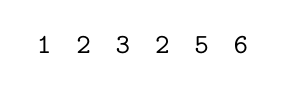
\begin{tikzpicture}
        \node at (.5, .25) {\texttt{1}};
        \node at (1, .25) {\texttt{2}};
        \node at (1.5, .25) {\texttt{3}};
        \node at (2, .25) {\texttt{2}};
        \node at (2.5, .25) {\texttt{5}};
        \node at (3, .25) {\texttt{6}};
    \end{tikzpicture}
\end{center}
The two sublists is now merged.

\noindent Since we iterate over all the elements, the merge algorithm is $O(n)$. Moreover, the procedure is stable, but not in place. It requires linear memory. Now, we consider the overall merge sort, using the merge procedure:
\begin{lstlisting}[language=pseudocode]
void mergeSort(Array<int> array, int p, int r):
    if (p < r):
        int q = (p + r)/2
        mergeSort(array, p, q)
        mergeSort(array, q+1, r)
        merge(array, p, q, r)
\end{lstlisting}
The merge sort divides the array, and aims to merge all the divided arrays. We can see how this function works by considering \texttt{mergeSort([0, 5, 6, 3, 2, 1, 3])}:
\begin{center}
    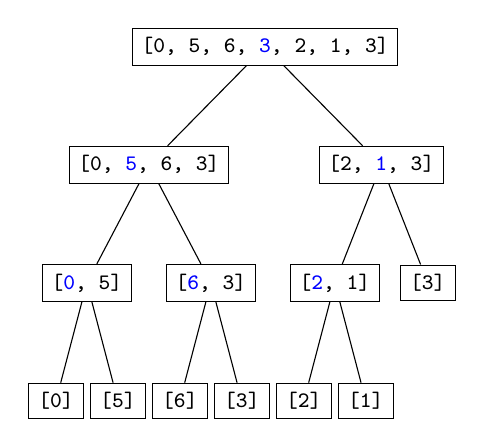
\begin{tikzpicture}
        \Tree[
        .\footnotesize\texttt{[0, 5, 6, {\color{blue}3}, 2, 1, 3]}
            [.\footnotesize\texttt{[0, {\color{blue}5}, 6, 3]}
                [.\footnotesize\texttt{[{\color{blue}0}, 5]}
                    [.\footnotesize\texttt{[0]}
                    ]
                    [.\footnotesize\texttt{[5]}
                    ]
                ]
                [.\footnotesize\texttt{[{\color{blue}6}, 3]}
                    [.\footnotesize\texttt{[6]}
                    ]
                    [.\footnotesize\texttt{[3]}
                    ]
                ]
            ]
            [.\footnotesize\texttt{[2, {\color{blue}1}, 3]}
                [.\footnotesize\texttt{[{\color{blue}2}, 1]}
                    [.\footnotesize\texttt{[2]}
                    ]
                    [.\footnotesize\texttt{[1]}
                    ]
                ]
                [.\footnotesize\texttt{[3]}
                ]
            ]
        ]
    \end{tikzpicture}
\end{center}
The element highlighted in blue is the value of \texttt{q}. After breaking all the elements, we merge the arrays to get \texttt{[0, 1, 2, 3, 3, 5, 6]}.

\noindent Like the merge algorithm, merge sort is stable and not in-place. Its running time is $O(n \log n)$ in both the best and the worst case. We can prove this using iterative substitution. The base case (i.e. $p \geq r$) has running time $T(1) = O(1)$, while the recursive case has running time $T(n) = T(n/2) + T(n/2) + O(n) = 2T(n/2) + O(n)$- the sorting of the smaller sublists is $T(n/2)$, while the merge is $O(n)$. We now substitute this iteratively:
\begin{align*}
    T(n) &= 2T(n/2) + O(n) \\
    &= 2(2T(n/4) + O(n/2)) + O(n) \\
    &= 4T(n/4) + 2O(n) \\
    &= 8T(n/8) + 3O(n) \\
    &= \cdots \\
    &= 2^k T(n/2^k) + kO(n).
\end{align*}
The base case happens when $n = 1$, i.e. $n = 2^k$. So, $k = \log n$, meaning that $T(n) = nO(1) + \log n O(n)$. This implies that merge sort is $n \log n$.

\noindent We could also have computed this using recursion tree. We would find that, at each level, we have running time of $O(n)$. Since the tree has height $\log n$, the running time of the entire method is therefore $O(n \log n)$.

\noindent Similarly, we can also use the Master theorem. In this case, we have $c = 1$ and $\log_2 2 = 1 = c$. So, $T(n) = \Theta(n \log n)$, as we found.

\noindent We can improve merge sort in many ways:
\begin{itemize}
    \item We can make the algorithm in place by amending the \texttt{merge} algorithm.
    \item We can make the \texttt{mergeSort} algorithm iterative.
    \item We can make use of \texttt{insertionSort} when the array size is small. Cutoffs are typically set between 5 and 20 elements.
\end{itemize}

\subsection{Quick sort}
Quick sort is another divide-and-conquer sorting algorithm. We choose a pivot element and the division aims to break an array into two sublists- one containing all the elements smaller than the pivot, while the other one contains all the elements bigger than the pivot. Doing this recursively ensures that we end up with a sorted array- there is no combination step. The following is the way we partition the array, choosing the pivot to be the last element.
\begin{lstlisting}[language=pseudocode]
int partition(Array<int> array, int p, int r):
    int x = array[r]
    int i = p-1
    for (int j = p; j < r; j++):
        if (array[j] <= x):
            i++
            array[i], array[j] = array[j], array[i]
    array[i], array[i+1] = array[i+1], array[i]
    return i+1
\end{lstlisting}
We illustrate how this algorithm works using the array \texttt{[0, 7, 5, 2, 4, 1, 3]} and \texttt{p=0}, \texttt{r=6}. We start with the following state:
\begin{center}
    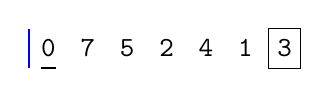
\begin{tikzpicture}
        \draw [thick] (.4, 0) -- (.6, 0);
        \draw [thick, blue] (.25, 0) -- (.25, .5);
        \node at (.5, .25) {\texttt{0}};
        \node at (1, .25) {\texttt{7}};
        \node at (1.5, .25) {\texttt{5}};
        \node at (2, .25) {\texttt{2}};
        \node at (2.5, .25) {\texttt{4}};
        \node at (3, .25) {\texttt{1}};
        \node at (3.5, .25) {\texttt{3}};
        \draw (3.3, 0) -- (3.3, .5) -- (3.7, .5) -- (3.7, 0) -- cycle;
    \end{tikzpicture}
\end{center}
The pivot \texttt{x} is the element in the box. The blue wall keeps track of the sublist that is smaller than the pivot and represents the variable \texttt{i}. Within the for loop, \texttt{j} is represented by an underline. When we first enter the while loop, we check whether \texttt{1} is smaller than the pivot- since \texttt{1} is smaller, we swap it with the first element after the blue wall, i.e. with itself. We then move the blue wall.
\begin{center}
    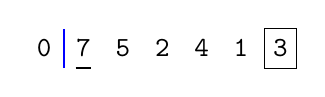
\begin{tikzpicture}
        \draw [thick] (.9, 0) -- (1.1, 0);
        \draw [thick, blue] (.75, 0) -- (.75, .5);
        \node at (.5, .25) {\texttt{0}};
        \node at (1, .25) {\texttt{7}};
        \node at (1.5, .25) {\texttt{5}};
        \node at (2, .25) {\texttt{2}};
        \node at (2.5, .25) {\texttt{4}};
        \node at (3, .25) {\texttt{1}};
        \node at (3.5, .25) {\texttt{3}};
        \draw (3.3, 0) -- (3.3, .5) -- (3.7, .5) -- (3.7, 0) -- cycle;
    \end{tikzpicture}
\end{center}
Now, we check whether \texttt{7} is smaller than the pivot- it isn't, so we just move onto the next element.
\begin{center}
    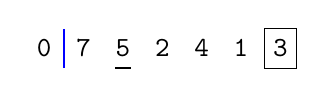
\begin{tikzpicture}
        \draw [thick] (1.4, 0) -- (1.6, 0);
        \draw [thick, blue] (.75, 0) -- (.75, .5);
        \node at (.5, .25) {\texttt{0}};
        \node at (1, .25) {\texttt{7}};
        \node at (1.5, .25) {\texttt{5}};
        \node at (2, .25) {\texttt{2}};
        \node at (2.5, .25) {\texttt{4}};
        \node at (3, .25) {\texttt{1}};
        \node at (3.5, .25) {\texttt{3}};
        \draw (3.3, 0) -- (3.3, .5) -- (3.7, .5) -- (3.7, 0) -- cycle;
    \end{tikzpicture}
\end{center}
Since \texttt{5} is also bigger than \texttt{3}, we do nothing in this iteration.
\begin{center}
    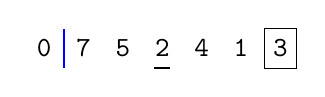
\begin{tikzpicture}
        \draw [thick] (1.9, 0) -- (2.1, 0);
        \draw [thick, blue] (.75, 0) -- (.75, .5);
        \node at (.5, .25) {\texttt{0}};
        \node at (1, .25) {\texttt{7}};
        \node at (1.5, .25) {\texttt{5}};
        \node at (2, .25) {\texttt{2}};
        \node at (2.5, .25) {\texttt{4}};
        \node at (3, .25) {\texttt{1}};
        \node at (3.5, .25) {\texttt{3}};
        \draw (3.3, 0) -- (3.3, .5) -- (3.7, .5) -- (3.7, 0) -- cycle;
    \end{tikzpicture}
\end{center}
Now, since \texttt{2} is smaller than the pivot, we swap it with the first element after the blue wall. We then increment the blue wall.
\begin{center}
    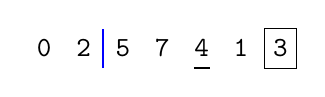
\begin{tikzpicture}
        \draw [thick] (2.4, 0) -- (2.6, 0);
        \draw [thick, blue] (1.25, 0) -- (1.25, .5);
        \node at (.5, .25) {\texttt{0}};
        \node at (1, .25) {\texttt{2}};
        \node at (1.5, .25) {\texttt{5}};
        \node at (2, .25) {\texttt{7}};
        \node at (2.5, .25) {\texttt{4}};
        \node at (3, .25) {\texttt{1}};
        \node at (3.5, .25) {\texttt{3}};
        \draw (3.3, 0) -- (3.3, .5) -- (3.7, .5) -- (3.7, 0) -- cycle;
    \end{tikzpicture}
\end{center}
As \texttt{4} is bigger than the pivot, nothing changes in this iteration.
\begin{center}
    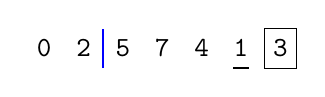
\begin{tikzpicture}
        \draw [thick] (2.9, 0) -- (3.1, 0);
        \draw [thick, blue] (1.25, 0) -- (1.25, .5);
        \node at (.5, .25) {\texttt{0}};
        \node at (1, .25) {\texttt{2}};
        \node at (1.5, .25) {\texttt{5}};
        \node at (2, .25) {\texttt{7}};
        \node at (2.5, .25) {\texttt{4}};
        \node at (3, .25) {\texttt{1}};
        \node at (3.5, .25) {\texttt{3}};
        \draw (3.3, 0) -- (3.3, .5) -- (3.7, .5) -- (3.7, 0) -- cycle;
    \end{tikzpicture}
\end{center}
In the final iteration, we swap \texttt{1} and \texttt{5}.
\begin{center}
    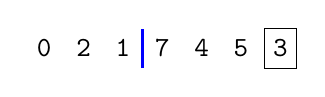
\begin{tikzpicture}
        \draw [thick, blue] (1.75, 0) -- (1.75, .5);
        \node at (.5, .25) {\texttt{0}};
        \node at (1, .25) {\texttt{2}};
        \node at (1.5, .25) {\texttt{1}};
        \node at (2, .25) {\texttt{7}};
        \node at (2.5, .25) {\texttt{4}};
        \node at (3, .25) {\texttt{5}};
        \node at (3.5, .25) {\texttt{3}};
        \draw (3.3, 0) -- (3.3, .5) -- (3.7, .5) -- (3.7, 0) -- cycle;
    \end{tikzpicture}
\end{center}
After exiting the while loop, we swap \texttt{3} with the first element after the blue wall to give the partitioned array.
\begin{center}
    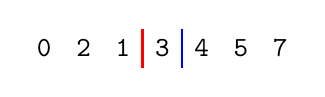
\begin{tikzpicture}
        \draw [thick, blue] (2.25, 0) -- (2.25, .5);
        \draw [thick, red] (1.75, 0) -- (1.75, .5);
        \node at (.5, .25) {\texttt{0}};
        \node at (1, .25) {\texttt{2}};
        \node at (1.5, .25) {\texttt{1}};
        \node at (2, .25) {\texttt{3}};
        \node at (2.5, .25) {\texttt{4}};
        \node at (3, .25) {\texttt{5}};
        \node at (3.5, .25) {\texttt{7}};
    \end{tikzpicture}
\end{center}
We now recursively partition the two sublists until we end up with a sorted array. The number returned gives us access to the start and the end of these sublists. 

\noindent The running time of the partition function is $O(n)$. The function is in place, but not stable. Using the algorithm, we can define the quicksort algorithm:
\begin{lstlisting}[language=pseudocode]
void quickSort(Array<int> array, int p, int r):
    if (p < r):
        int q = partition(array, p, r)
        quickSort(array, p, q-1)
        quickSort(array, q+1, r)
\end{lstlisting}
The recursion tree for the array \texttt{[6, 5, 0, 4, 1, 8, 3]} is:
\begin{center}
    \Tree[
    .\footnotesize\texttt{[6, 5, 0, 4, 1, 8, {\color{red}3}]}
        [.\footnotesize\texttt{[0, {\color{red}1}]}
            [.\footnotesize\texttt{[0]}
            ]
        ]
        [.\footnotesize\texttt{[4, 5, 8, {\color{red}6}]}
            [.\footnotesize\texttt{[4, {\color{red}5}]}
                [.\footnotesize\texttt{[4]}
                ]
            ]
            [.\footnotesize\texttt{[8]}
            ]
        ]
    ]
\end{center}
The element highlighted in red is the pivot. 

\noindent The running time of median depends on the choice of the pivot. In the best case, the pivot is always the median. Then, the recurrence equation is $T(n) = 2T(n/2) + O(n)$. This is the same equation as merge sort, so it is $O(n \log n)$. On the other hand, if we are at the worst case, the pivot is very unbalanced- we end up with one sublist of size \texttt{n-1} and another of size \texttt{0}. The recurrence equation in that case is
\[T(n) = T(n-1) + T(0) + O(n) = T(n-1) + O(n)\]
since $T(0) = O(1)$. We find that
\begin{align*}
    T(n) &= T(n-1) + O(n) \\
    &= T(n-2) + 2O(n) \\
    &= \cdots \\
    &= T(0) + nO(n).
\end{align*}
So, $T(n) = O(n^2)$. This only happens when the array is already sorted. On average, the algorithm is $O(n \log n)$.

\noindent We could make the algorithm better by choosing a different element, e.g. the middle. This could still degrade to $O(n^2)$. We can also consider the median of 3 numbers- the start, the middle and the end. It is a bit slower, and we could still degrade to $O(n^2)$. We could also choose the pivot randomly, although that is not always feasible/fast.

\noindent We can use a cutoff like in the case of merge sort. Here, we call insertion sort on the entire array- insertion sort performs better with nearly sorted arrays. We can tail-optimise and then we only have one recursion call. We can also make the quicksort iterative.

\noindent Finally, we can use a 3-way quicksort, where we have a third sublist containing all the elements equal to the pivot. It is a good algorithm if there are many duplicates.

\subsection{Heap sort}
Heap sort is an iterative algorithm that makes use of the heap data structure in order to sort the array. It iteratively extracts the maximum element from the unsorted sublist. Unlike selection sort, it is better because the heap data structure makes the search a linear operation. 

\noindent A heap is a nearly complete binary tree that satisfies the heap property- if \texttt{p} is a parent node of \texttt{c}, then the value of \texttt{p} is greater than or equal to the value of \texttt{c}. We can implement a heap as an array. For example, the following represents a heap:
\begin{center}
    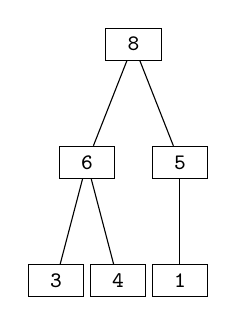
\begin{tikzpicture}
        \Tree[.\footnotesize\texttt{8}
            [.\footnotesize\texttt{6}
                [.\footnotesize\texttt{3}
                ]
                [.\footnotesize\texttt{4}
                ]
            ]
            [.\footnotesize\texttt{5}
                [.\footnotesize\texttt{1}
                ]
            ]
        ]
    \end{tikzpicture} 
\end{center}
Here, we always find that the parent node of an element is bigger than the element, and vice versa. The heap is called nearly complete since all the level, except for the final one, are complete. We store it as an array going top to bottom and then from left to right. In this case, the array will be:
\begin{center}
    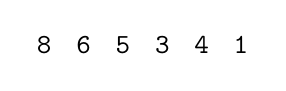
\begin{tikzpicture}
        \node at (-1.5, -3.75) {\texttt{8}};
        \node at (-1, -3.75) {\texttt{6}};
        \node at (-.5, -3.75) {\texttt{5}};
        \node at (0, -3.75) {\texttt{3}};
        \node at (.5, -3.75) {\texttt{4}};
        \node at (1, -3.75) {\texttt{1}};
    \end{tikzpicture}
\end{center}
For an element in the array, its left child is in index $2n + 1$ while its right child is at index $2n + 2$.

\noindent Now, we consider the algorithm for heapsort. The pseudocode is:
\begin{lstlisting}[language=pseudocode]
void heapSort(Array<int> array):
    createHeap(array)
    for (int i = array.length-1; i >= 0; i--):
        array[0], array[i] = array[i], array[0]
        heapify(array, 0, i)
\end{lstlisting}
First, we aim to transform an array into a heap structure. As a heap, we know that the maximum element is at the start. So, we swap it with the last element in the unsorted (left) sublist. Then, we re-establish the heap structure in the array and continue finding the maximum element.

\noindent We now consider how the algorithm works with the array \texttt{[3, 5, 2, 0, 9, 7]}.
\begin{center}
    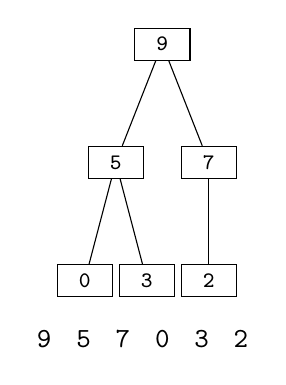
\begin{tikzpicture}
        \Tree[.\footnotesize\texttt{9}
            [.\footnotesize\texttt{5}
                [.\footnotesize\texttt{0}
                ]
                [.\footnotesize\texttt{3}
                ]
            ]
            [.\footnotesize\texttt{7}
                [.\footnotesize\texttt{2}
                ]
            ]
        ]
        \node at (-1.5, -3.75) {\texttt{9}};
        \node at (-1, -3.75) {\texttt{5}};
        \node at (-.5, -3.75) {\texttt{7}};
        \node at (0, -3.75) {\texttt{0}};
        \node at (.5, -3.75) {\texttt{3}};
        \node at (1, -3.75) {\texttt{2}};
    \end{tikzpicture} 
\end{center}
First, we transform the array into a heap.
\begin{center}
    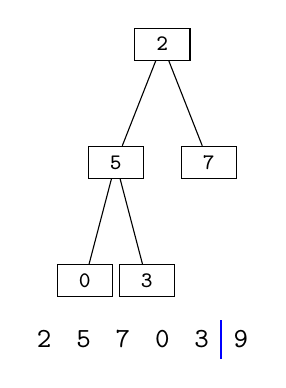
\begin{tikzpicture}
        \Tree[.\footnotesize\texttt{2}
            [.\footnotesize\texttt{5}
                [.\footnotesize\texttt{0}
                ]
                [.\footnotesize\texttt{3}
                ]
            ]
            [.\footnotesize\texttt{7}
            ]
        ]
        \draw[thick, blue] (0.75, -4) -- (0.75, -3.5);
        \node at (-1.5, -3.75) {\texttt{2}};
        \node at (-1, -3.75) {\texttt{5}};
        \node at (-.5, -3.75) {\texttt{7}};
        \node at (0, -3.75) {\texttt{0}};
        \node at (.5, -3.75) {\texttt{3}};
        \node at (1, -3.75) {\texttt{9}};
    \end{tikzpicture} 
\end{center}
Now, we enter the for loop. The first thing we do is swap the first element \texttt{9} with the element at the end of the unsorted sublist (blue wall) \texttt{3}. The heap now has one fewer element.
\begin{center}
    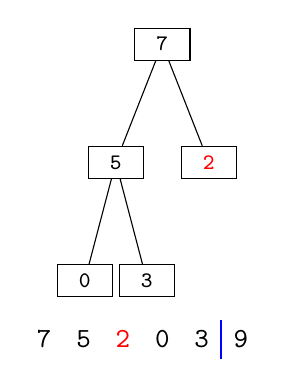
\begin{tikzpicture}
        \Tree[.\footnotesize\texttt{7}
            [.\footnotesize\texttt{5}
                [.\footnotesize\texttt{0}
                ]
                [.\footnotesize\texttt{3}
                ]
            ]
            [.\footnotesize\texttt{\color{red}2}
            ]
        ]
        \draw[thick, blue] (0.75, -4) -- (0.75, -3.5);
        \node at (-1.5, -3.75) {\texttt{7}};
        \node at (-1, -3.75) {\texttt{5}};
        \node[color=red] at (-.5, -3.75) {\texttt{2}};
        \node at (0, -3.75) {\texttt{0}};
        \node at (.5, -3.75) {\texttt{3}};
        \node at (1, -3.75) {\texttt{9}};
    \end{tikzpicture} 
\end{center}
We then restore the heap structure to the array.
\begin{center}
    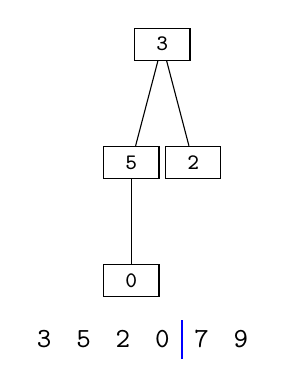
\begin{tikzpicture}
        \Tree[.\footnotesize\texttt{3}
            [.\footnotesize\texttt{5}
                [.\footnotesize\texttt{0}
                ]
            ]
            [.\footnotesize\texttt{2}
            ]
        ]
        \draw[thick, blue] (0.25, -4) -- (0.25, -3.5);
        \node at (-1.5, -3.75) {\texttt{3}};
        \node at (-1, -3.75) {\texttt{5}};
        \node at (-.5, -3.75) {\texttt{2}};
        \node at (0, -3.75) {\texttt{0}};
        \node at (.5, -3.75) {\texttt{7}};
        \node at (1, -3.75) {\texttt{9}};
    \end{tikzpicture} 
\end{center}
Next, we swap \texttt{7} and \texttt{3} and expand the sorted sublist.
\begin{center}
    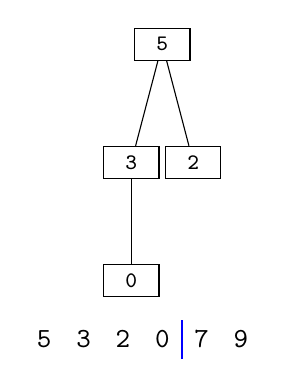
\begin{tikzpicture}
        \Tree[.\footnotesize\texttt{5}
            [.\footnotesize\texttt{3}
                [.\footnotesize\texttt{0}
                ]
            ]
            [.\footnotesize\texttt{2}
            ]
        ]
        \draw[thick, blue] (0.25, -4) -- (0.25, -3.5);
        \node at (-1.5, -3.75) {\texttt{5}};
        \node at (-1, -3.75) {\texttt{3}};
        \node at (-.5, -3.75) {\texttt{2}};
        \node at (0, -3.75) {\texttt{0}};
        \node at (.5, -3.75) {\texttt{7}};
        \node at (1, -3.75) {\texttt{9}};
    \end{tikzpicture} 
\end{center}
Again, we restore the heap structure.
\begin{center}
    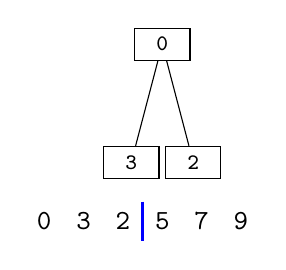
\begin{tikzpicture}
        \Tree[.\footnotesize\texttt{0}
            [.\footnotesize\texttt{3}
            ]
            [.\footnotesize\texttt{2}
            ]
        ]
        \draw[thick, blue] (-0.25, -2) -- (-0.25, -2.5);
        \node at (-1.5, -2.25) {\texttt{0}};
        \node at (-1, -2.25) {\texttt{3}};
        \node at (-.5, -2.25) {\texttt{2}};
        \node at (0, -2.25) {\texttt{5}};
        \node at (.5, -2.25) {\texttt{7}};
        \node at (1, -2.25) {\texttt{9}};
    \end{tikzpicture} 
\end{center}
We now swap the maximum element \texttt{5} with \texttt{0}.
\begin{center}
    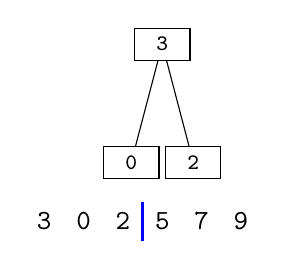
\begin{tikzpicture}
        \Tree[.\footnotesize\texttt{3}
            [.\footnotesize\texttt{0}
            ]
            [.\footnotesize\texttt{2}
            ]
        ]
        \draw[thick, blue] (-0.25, -2) -- (-0.25, -2.5);
        \node at (-1.5, -2.25) {\texttt{3}};
        \node at (-1, -2.25) {\texttt{0}};
        \node at (-.5, -2.25) {\texttt{2}};
        \node at (0, -2.25) {\texttt{5}};
        \node at (.5, -2.25) {\texttt{7}};
        \node at (1, -2.25) {\texttt{9}};
    \end{tikzpicture} 
\end{center}
Again, we restore the heap property.
\begin{center}
    \begin{tikzpicture}
        \Tree[.\footnotesize\texttt{2}
            [.\footnotesize\texttt{0}
            ]
        ]
        \draw[thick, blue] (-0.75, -2) -- (-0.75, -2.5);
        \node at (-1.5, -2.25) {\texttt{2}};
        \node at (-1, -2.25) {\texttt{0}};
        \node at (-.5, -2.25) {\texttt{3}};
        \node at (0, -2.25) {\texttt{5}};
        \node at (.5, -2.25) {\texttt{7}};
        \node at (1, -2.25) {\texttt{9}};
    \end{tikzpicture} 
\end{center}
Now, we swap \texttt{3} and \texttt{2}. This configuration still obeys the heap structure.
\begin{center}
    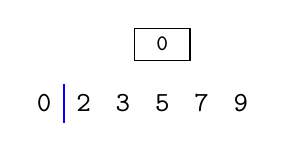
\begin{tikzpicture}
        \Tree[.\footnotesize\texttt{0}
        ]
        \draw[thick, blue] (-1.25, -0.5) -- (-1.25, -1);
        \node at (-1.5, -0.75) {\texttt{0}};
        \node at (-1, -0.75) {\texttt{2}};
        \node at (-.5, -0.75) {\texttt{3}};
        \node at (0, -0.75) {\texttt{5}};
        \node at (.5, -0.75) {\texttt{7}};
        \node at (1, -0.75) {\texttt{9}};
    \end{tikzpicture} 
\end{center}
Finally, we have arrived at a heap with height 1. This implies that the array is sorted. So, the sort gives us
\begin{center}
    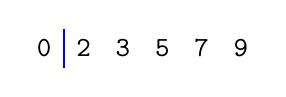
\begin{tikzpicture}
        \draw[thick, blue] (-1.25, -0.5) -- (-1.25, -1);
        \node at (-1.5, -0.75) {\texttt{0}};
        \node at (-1, -0.75) {\texttt{2}};
        \node at (-.5, -0.75) {\texttt{3}};
        \node at (0, -0.75) {\texttt{5}};
        \node at (.5, -0.75) {\texttt{7}};
        \node at (1, -0.75) {\texttt{9}};
    \end{tikzpicture} 
\end{center}
The algorithm is analogous to a variant of selection sort. Now, we consider the algorithms \texttt{heapify} that restores the heap structure. 
\begin{lstlisting}[language=pseudocode]
void heapify(Array<int> array, int i, int length):
    int left = 2*i + 1
    int right = 2*i + 2
    int largest = null
    // left bigger than parent -> the largest is left child
    if (left < length && array[left] > array[i]):
        largest = left
    else:
        largest = i
    // right bigger than left/parent -> the largest is right child
    if (right < length && array[right] > array[largest]):
        largest = right
    // swap largest with i and recurse if different
    if (largest != i):
        array[i], array[largest] = array[largest], array[i]
        heapify(array, largest, length)
\end{lstlisting}
It checks whether the left or the right child is larger than the element- if it is, we swap the child with the parent, and recurse on that child to ensure the heap structure is still satisfied.

\noindent Also, the function \texttt{createHeap} makes use of \texttt{heapify} to convert the array into a heap.
\begin{lstlisting}[language=pseudocode]
void createHeap(Array<int> array):
    for (int i = (array.length/2) - 1; i >= 0; i--):
        array[0], array[i] = array[i], array[0]
        heapify(array, 0, i)
\end{lstlisting}
We now consider how we create the heap structure for the array \texttt{[3, 5, 2, 0, 9, 7]}.
\begin{center}
    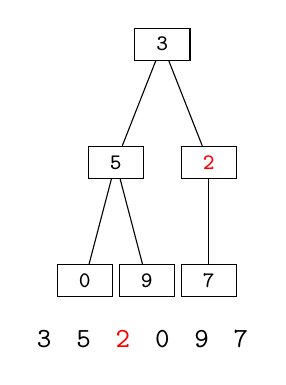
\begin{tikzpicture}
        \Tree[.\footnotesize\texttt{3}
            [.\footnotesize\texttt{5}
                [.\footnotesize\texttt{0}
                ]
                [.\footnotesize\texttt{9}
                ]
            ]
            [.\footnotesize\texttt{\color{red}2}
                [.\footnotesize\texttt{7}
                ]
            ]
        ]
        \node at (-1.5, -3.75) {\texttt{3}};
        \node at (-1, -3.75) {\texttt{5}};
        \node[color=red] at (-.5, -3.75) {\texttt{2}};
        \node at (0, -3.75) {\texttt{0}};
        \node at (.5, -3.75) {\texttt{9}};
        \node at (1, -3.75) {\texttt{7}};
    \end{tikzpicture} 
\end{center}
Originally, the array doesn't satisfy the heap property. We enter the for loop and ensure the indices \texttt{2}, \texttt{1} and \texttt{0} satisfy the heap property. We start with index \texttt{2}. Since the (left) child of \texttt{2} is bigger, we swap the two elements.
\begin{center}
    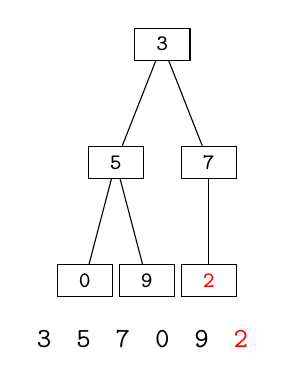
\begin{tikzpicture}
        \Tree[.\footnotesize\texttt{3}
            [.\footnotesize\texttt{5}
                [.\footnotesize\texttt{0}
                ]
                [.\footnotesize\texttt{9}
                ]
            ]
            [.\footnotesize\texttt{7}
                [.\footnotesize\texttt{\color{red}2}
                ]
            ]
        ]
        \node at (-1.5, -3.75) {\texttt{3}};
        \node at (-1, -3.75) {\texttt{5}};
        \node at (-.5, -3.75) {\texttt{7}};
        \node at (0, -3.75) {\texttt{0}};
        \node at (.5, -3.75) {\texttt{9}};
        \node[color=red] at (1, -3.75) {\texttt{2}};
    \end{tikzpicture} 
\end{center}
Now, we ensure that \texttt{2} satisfies the heap property. It has no children, so there is nothing to check here.
\begin{center}
    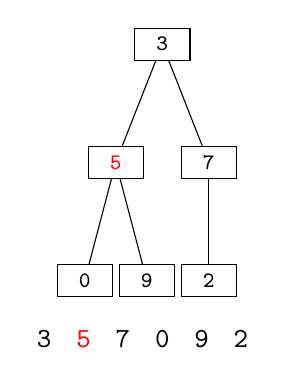
\begin{tikzpicture}
        \Tree[.\footnotesize\texttt{3}
            [.\footnotesize\texttt{\color{red}5}
                [.\footnotesize\texttt{0}
                ]
                [.\footnotesize\texttt{9}
                ]
            ]
            [.\footnotesize\texttt{7}
                [.\footnotesize\texttt{2}
                ]
            ]
        ]
        \node at (-1.5, -3.75) {\texttt{3}};
        \node[color=red] at (-1, -3.75) {\texttt{5}};
        \node at (-.5, -3.75) {\texttt{7}};
        \node at (0, -3.75) {\texttt{0}};
        \node at (.5, -3.75) {\texttt{9}};
        \node at (1, -3.75) {\texttt{2}};
    \end{tikzpicture} 
\end{center}
Now, we move onto index \texttt{1}. The right child of \texttt{5} is bigger, so we swap the two elements.
\begin{center}
    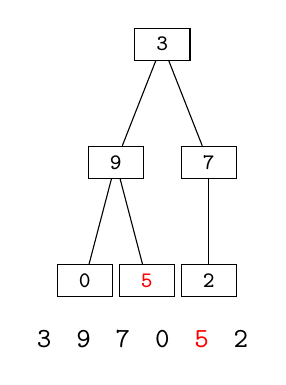
\begin{tikzpicture}
        \Tree[.\footnotesize\texttt{3}
            [.\footnotesize\texttt{9}
                [.\footnotesize\texttt{0}
                ]
                [.\footnotesize\texttt{\color{red}5}
                ]
            ]
            [.\footnotesize\texttt{7}
                [.\footnotesize\texttt{2}
                ]
            ]
        ]
        \node at (-1.5, -3.75) {\texttt{3}};
        \node at (-1, -3.75) {\texttt{9}};
        \node at (-.5, -3.75) {\texttt{7}};
        \node at (0, -3.75) {\texttt{0}};
        \node[color=red] at (.5, -3.75) {\texttt{5}};
        \node at (1, -3.75) {\texttt{2}};
    \end{tikzpicture} 
\end{center}
The element \texttt{5} has no children, so there is nothing to check here.
\begin{center}
    \begin{tikzpicture}
        \Tree[.\footnotesize\texttt{\color{red}3}
            [.\footnotesize\texttt{9}
                [.\footnotesize\texttt{0}
                ]
                [.\footnotesize\texttt{5}
                ]
            ]
            [.\footnotesize\texttt{7}
                [.\footnotesize\texttt{2}
                ]
            ]
        ]
        \node[color=red] at (-1.5, -3.75) {\texttt{3}};
        \node at (-1, -3.75) {\texttt{9}};
        \node at (-.5, -3.75) {\texttt{7}};
        \node at (0, -3.75) {\texttt{0}};
        \node at (.5, -3.75) {\texttt{5}};
        \node at (1, -3.75) {\texttt{2}};
    \end{tikzpicture} 
\end{center}
Finally, we move onto applying the \texttt{heapify} function on index \texttt{0}. \texttt{3} is smaller than both \texttt{7} and \texttt{9}, but \texttt{9} is bigger than the other child. So, we swap \texttt{3} and \texttt{9}.
\begin{center}
    \begin{tikzpicture}
        \Tree[.\footnotesize\texttt{9}
            [.\footnotesize\texttt{\color{red}3}
                [.\footnotesize\texttt{0}
                ]
                [.\footnotesize\texttt{5}
                ]
            ]
            [.\footnotesize\texttt{7}
                [.\footnotesize\texttt{2}
                ]
            ]
        ]
        \node at (-1.5, -3.75) {\texttt{9}};
        \node[color=red] at (-1, -3.75) {\texttt{3}};
        \node at (-.5, -3.75) {\texttt{7}};
        \node at (0, -3.75) {\texttt{0}};
        \node at (.5, -3.75) {\texttt{5}};
        \node at (1, -3.75) {\texttt{2}};
    \end{tikzpicture} 
\end{center}
\texttt{3} is smaller than \texttt{5}, so we swap them.
\begin{center}
    \begin{tikzpicture}
        \Tree[.\footnotesize\texttt{9}
            [.\footnotesize\texttt{5}
                [.\footnotesize\texttt{0}
                ]
                [.\footnotesize\texttt{\color{red}3}
                ]
            ]
            [.\footnotesize\texttt{7}
                [.\footnotesize\texttt{2}
                ]
            ]
        ]
        \node at (-1.5, -3.75) {\texttt{9}};
        \node at (-1, -3.75) {\texttt{5}};
        \node at (-.5, -3.75) {\texttt{7}};
        \node at (0, -3.75) {\texttt{0}};
        \node[color=red] at (.5, -3.75) {\texttt{3}};
        \node at (1, -3.75) {\texttt{2}};
    \end{tikzpicture} 
\end{center}
Since \texttt{3} has no children, there is nothing more to check. We have acheived the heap structure.

\noindent The function \texttt{createHeap} is $O(n)$. The function \texttt{heapify} is $O(\log n)$- this is an improvement from the $O(n)$ version in selection sort. Since there are \texttt{n-1} iterations, the complexity of the algorithm is $O(n \log n)$. This is in both the best and the worst case. The algorithm is in place, but not stable.

\subsection{Non-comparison Sorts}
All the sorting algorithms we've looked at have been comparison sorts. That is, we compare elements to determine the permutation of the array that gives us a sorted array. We can consider all comparison sorts abstractly as a decision tree model. We only look at the comparisons in that case. 

\noindent A decision tree is a complete binary tree that represents comparisons between the elements with respect to the input size. We expect the elements within the array to be distinct. Using the binary tree, we can find a lower bound to comparison sorts. For example, for an array of 3 elements, the decision tree is:
\begin{center}
    \begin{tikzpicture}
        \Tree[
        .\footnotesize\texttt{0:1}
            [.\footnotesize\texttt{1:2}
                [.\footnotesize\texttt{[0,1,2}]
                ]
                [.\footnotesize\texttt{0:2}
                    [.\footnotesize\texttt{[0,2,1]}
                    ]
                    [.\footnotesize\texttt{[2,0,1]}
                    ]
                ]
            ]
            [.\footnotesize\texttt{0:2}
                [.\footnotesize\texttt{[1,0,2]}
                ]
                [.\footnotesize\texttt{1:2}
                    [.\footnotesize\texttt{[1,2,0]}
                    ]
                    [.\footnotesize\texttt{[2,1,0]}
                    ]
                ]
            ]
        ]
    \end{tikzpicture}
\end{center}
We only indicate the indices above. The leaf nodes represent the indices of the sorted array, while all the other nodes are decision nodes. For a condition \texttt{a:b}, if we go to the left, we have \texttt{a <= b}. On the other hand, if we go to the right, \texttt{a > b}. Depending on the comparisons, we can end up with all the 6 possible permutations of the three elements. 

\noindent For a comparison sort, it must be possible to go down every path. Therefore, the worst running time is the height of the decision tree. We know that $n^{n/2} \leq n! \leq n^n$, and that a binary tree of height $h$ has at most $2^h$ leaves. Therefore,
\[h \geq \log (n!) \geq \log (n^{n/2}) = \frac{n}{2} \log n = \Omega(n \log n).\]
That is, a comparison sort has at lowest $O(n \log n)$. We say that merge sort and heapsort are asymptotically optimal- it is possible to improve these algorithms just by a comparison factor.

\subsubsection{Counting sort}
In search for a better running time, we now look at non-comparison sorts. Counting sort is an efficient sorting algorithm for integers between $0$ and $k$. Its running time is $O(n+k)$- it is linear since it has no comparisons. Moreover, it is a stable algorithm. It requires additional $O(n+k)$ memory. The pseudocode for counting sort is given below:
\begin{lstlisting}[language=pseudocode]
Array<int> countingSort(Array<int> array, int k):
    Array<int> count = []
    // we initialise the array count with zeros
    for (int i = 0; i < k; i++):
        count.add(0)
    Array<int> sorted = []
    // we also initialise the array sorted with zeros
    for (int i = 0; i < array.length; i++):
        sorted.add(0)
    // count the values between 0 and k-1 in the array
    for (int i = 0; j < array.length; j++):
        count[array[i]]++
    // update the count to make it accumulative
    for (int i = 1; i < k; i++):
        count[i] += count[i-1]
    // add to the sorted while updating the count
    for (int i = n-1; i >= 0; i--):
        sorted[count[array[i]]-1] = array[i]
        count[array[i]]--
    return sorted
\end{lstlisting}
There are 3 parts to the algorithm: we first count the occurrences of each number between 0 and k; we then make the array cumulative; and finally we copy the values into a new array. Clearly, there are no comparisons here.

\noindent We illustrate how the algorithm works by sorting the array \texttt{[1, 3, 7, 1, 4, 2]} with \texttt{k=7}. The first step is counting the number of elements between 0 and 7 in the array:
\begin{center}
    \begin{tikzpicture}
        \node at (-.8, .25) {\texttt{array}};
        \node at (0, .25) {\texttt{1}};
        \node at (.5, .25) {\texttt{3}};
        \node at (1, .25) {\texttt{7}};
        \node at (1.5, .25) {\texttt{1}};
        \node at (2, .25) {\texttt{4}};
        \node at (2.5, .25) {\texttt{2}};
        
        \node at (-.8, -.25) {\texttt{count}};
        \node at (0, -.25) {\texttt{0}};
        \node at (.5, -.25) {\texttt{2}};
        \node at (1, -.25) {\texttt{1}};
        \node at (1.5, -.25) {\texttt{1}};
        \node at (2, -.25) {\texttt{1}};
        \node at (2.5, -.25) {\texttt{0}};
        \node at (3, -.25) {\texttt{0}};
        \node at (3.5, -.25) {\texttt{1}};
    \end{tikzpicture}
\end{center}
We traverse through the \texttt{array} and increment the array \texttt{count} at the relevant index if we encounter an element with that value. The array \texttt{count} states that there are no 0; two 1; one 2; one 3; one 4; no 5; no 6; and one 7. Now, we make the count cumulative:
\begin{center}
    \begin{tikzpicture}
        \node at (-.8, -.25) {\texttt{count}};
        \node at (0, -.25) {\texttt{0}};
        \node at (.5, -.25) {\texttt{2}};
        \node at (1, -.25) {\texttt{3}};
        \node at (1.5, -.25) {\texttt{4}};
        \node at (2, -.25) {\texttt{5}};
        \node at (2.5, -.25) {\texttt{5}};
        \node at (3, -.25) {\texttt{5}};
        \node at (3.5, -.25) {\texttt{6}};
    \end{tikzpicture}
\end{center}
Using these values, we can now correctly index and place the elements within the array \texttt{sorted}.
\begin{center}
    \begin{tikzpicture}
        \node at (-.8, .25) {\texttt{array}};
        \draw[thick] (2.4, 0) -- (2.6, 0);
        \node at (0, .25) {\texttt{1}};
        \node at (.5, .25) {\texttt{3}};
        \node at (1, .25) {\texttt{7}};
        \node at (1.5, .25) {\texttt{1}};
        \node at (2, .25) {\texttt{4}};
        \node at (2.5, .25) {\texttt{2}};
        
        \node at (-.8, -.25) {\texttt{count}};
        \draw[thick] (.9, -.5) -- (1.1, -.5);
        \node at (0, -.25) {\texttt{0}};
        \node at (.5, -.25) {\texttt{2}};
        \node at (1, -.25) {\texttt{3}};
        \node at (1.5, -.25) {\texttt{4}};
        \node at (2, -.25) {\texttt{5}};
        \node at (2.5, -.25) {\texttt{5}};
        \node at (3, -.25) {\texttt{5}};
        \node at (3.5, -.25) {\texttt{6}};
        
        \node at (-.8, -.75) {\texttt{sorted}};
        \draw[thick] (-.1, -1) -- (.1, -1);
        \draw[thick] (.4, -1) -- (.6, -1);
        \draw[thick] (.9, -1) -- (1.1, -1);
        \draw[thick] (1.4, -1) -- (1.6, -1);
        \draw[thick] (1.9, -1) -- (2.1, -1);
        \draw[thick] (2.4, -1) -- (2.6, -1);
    \end{tikzpicture}
\end{center}
We traverse the \texttt{array} from the end. Since the element is \texttt{2}, we find the value of \texttt{count[2]=3}- it is \texttt{3}. So, we place the number \texttt{2} at position \texttt{3-1=2} in \texttt{sorted} and decremented \texttt{count[2]}.
\begin{center}
    \begin{tikzpicture}
        \node at (-.8, .25) {\texttt{array}};
        \draw[thick] (1.9, 0) -- (2.1, 0);
        \node at (0, .25) {\texttt{1}};
        \node at (.5, .25) {\texttt{3}};
        \node at (1, .25) {\texttt{7}};
        \node at (1.5, .25) {\texttt{1}};
        \node at (2, .25) {\texttt{4}};
        \node at (2.5, .25) {\texttt{2}};
        
        \node at (-.8, -.25) {\texttt{count}};
        \draw[thick] (1.9, -.5) -- (2.1, -.5);
        \node at (0, -.25) {\texttt{0}};
        \node at (.5, -.25) {\texttt{2}};
        \node at (1, -.25) {\texttt{2}};
        \node at (1.5, -.25) {\texttt{4}};
        \node at (2, -.25) {\texttt{5}};
        \node at (2.5, -.25) {\texttt{5}};
        \node at (3, -.25) {\texttt{5}};
        \node at (3.5, -.25) {\texttt{6}};
        
        \node at (-.8, -.75) {\texttt{sorted}};
        \draw[thick] (-.1, -1) -- (.1, -1);
        \draw[thick] (.4, -1) -- (.6, -1);
        \node at (1, -.75) {\texttt{2}};
        \draw[thick] (1.4, -1) -- (1.6, -1);
        \draw[thick] (1.9, -1) -- (2.1, -1);
        \draw[thick] (2.4, -1) -- (2.6, -1);
    \end{tikzpicture}
\end{center}
Now, we place the element \texttt{4} in the array \texttt{sorted}. Going by the \texttt{count}, we find that it should be placed at position \texttt{4}. We then decrement the value in the array \texttt{count}.
\begin{center}
    \begin{tikzpicture}
        \node at (-.8, .25) {\texttt{array}};
        \draw[thick] (1.4, 0) -- (1.6, 0);
        \node at (0, .25) {\texttt{1}};
        \node at (.5, .25) {\texttt{3}};
        \node at (1, .25) {\texttt{7}};
        \node at (1.5, .25) {\texttt{1}};
        \node at (2, .25) {\texttt{4}};
        \node at (2.5, .25) {\texttt{2}};
        
        \node at (-.8, -.25) {\texttt{count}};
        \draw[thick] (.4, -.5) -- (.6, -.5);
        \node at (0, -.25) {\texttt{0}};
        \node at (.5, -.25) {\texttt{2}};
        \node at (1, -.25) {\texttt{2}};
        \node at (1.5, -.25) {\texttt{4}};
        \node at (2, -.25) {\texttt{4}};
        \node at (2.5, -.25) {\texttt{5}};
        \node at (3, -.25) {\texttt{5}};
        \node at (3.5, -.25) {\texttt{6}};
        
        \node at (-.8, -.75) {\texttt{sorted}};
        \draw[thick] (-.1, -1) -- (.1, -1);
        \draw[thick] (.4, -1) -- (.6, -1);
        \node at (1, -.75) {\texttt{2}};
        \draw[thick] (1.4, -1) -- (1.6, -1);
        \node at (2, -.75) {\texttt{4}};
        \draw[thick] (2.4, -1) -- (2.6, -1);
    \end{tikzpicture}
\end{center}
Then, we place the element \texttt{1} in \texttt{sorted}. We need to place \texttt{1} in index \texttt{count[1]-1 =1}.
\begin{center}
    \begin{tikzpicture}
        \node at (-.8, .25) {\texttt{array}};
        \draw[thick] (.9, 0) -- (1.1, 0);
        \node at (0, .25) {\texttt{1}};
        \node at (.5, .25) {\texttt{3}};
        \node at (1, .25) {\texttt{7}};
        \node at (1.5, .25) {\texttt{1}};
        \node at (2, .25) {\texttt{4}};
        \node at (2.5, .25) {\texttt{2}};
        
        \node at (-.8, -.25) {\texttt{count}};
        \draw[thick] (3.4, -.5) -- (3.6, -.5);
        \node at (0, -.25) {\texttt{0}};
        \node at (.5, -.25) {\texttt{1}};
        \node at (1, -.25) {\texttt{2}};
        \node at (1.5, -.25) {\texttt{4}};
        \node at (2, -.25) {\texttt{4}};
        \node at (2.5, -.25) {\texttt{5}};
        \node at (3, -.25) {\texttt{5}};
        \node at (3.5, -.25) {\texttt{6}};
        
        \node at (-.8, -.75) {\texttt{sorted}};
        \draw[thick] (-.1, -1) -- (.1, -1);
        \node at (0.5, -.75) {\texttt{1}};
        \node at (1, -.75) {\texttt{2}};
        \draw[thick] (1.4, -1) -- (1.6, -1);
        \node at (2, -.75) {\texttt{4}};
        \draw[thick] (2.4, -1) -- (2.6, -1);
    \end{tikzpicture}
\end{center}
Now, we add \texttt{7} to \texttt{sorted}. We place it in index \texttt{counted[7]-1=5}.
\begin{center}
    \begin{tikzpicture}
        \node at (-.8, .25) {\texttt{array}};
        \draw[thick] (.4, 0) -- (.6, 0);
        \node at (0, .25) {\texttt{1}};
        \node at (.5, .25) {\texttt{3}};
        \node at (1, .25) {\texttt{7}};
        \node at (1.5, .25) {\texttt{1}};
        \node at (2, .25) {\texttt{4}};
        \node at (2.5, .25) {\texttt{2}};
        
        \node at (-.8, -.25) {\texttt{count}};
        \draw[thick] (1.4, -.5) -- (1.6, -.5);
        \node at (0, -.25) {\texttt{0}};
        \node at (.5, -.25) {\texttt{1}};
        \node at (1, -.25) {\texttt{2}};
        \node at (1.5, -.25) {\texttt{4}};
        \node at (2, -.25) {\texttt{4}};
        \node at (2.5, -.25) {\texttt{5}};
        \node at (3, -.25) {\texttt{5}};
        \node at (3.5, -.25) {\texttt{5}};
        
        \node at (-.8, -.75) {\texttt{sorted}};
        \draw[thick] (-.1, -1) -- (.1, -1);
        \node at (0.5, -.75) {\texttt{1}};
        \node at (1, -.75) {\texttt{2}};
        \draw[thick] (1.4, -1) -- (1.6, -1);
        \node at (2, -.75) {\texttt{4}};
        \node at (2.5, -.75) {\texttt{7}};
    \end{tikzpicture}
\end{center}
Now, we add to the array \texttt{sorted} \texttt{3} at index \texttt{3}.
\begin{center}
    \begin{tikzpicture}
        \node at (-.8, .25) {\texttt{array}};
        \draw[thick] (-.1, 0) -- (.1, 0);
        \node at (0, .25) {\texttt{1}};
        \node at (.5, .25) {\texttt{3}};
        \node at (1, .25) {\texttt{7}};
        \node at (1.5, .25) {\texttt{1}};
        \node at (2, .25) {\texttt{4}};
        \node at (2.5, .25) {\texttt{2}};
        
        \node at (-.8, -.25) {\texttt{count}};
        \draw[thick] (.4, -.5) -- (.6, -.5);
        \node at (0, -.25) {\texttt{0}};
        \node at (.5, -.25) {\texttt{1}};
        \node at (1, -.25) {\texttt{2}};
        \node at (1.5, -.25) {\texttt{3}};
        \node at (2, -.25) {\texttt{4}};
        \node at (2.5, -.25) {\texttt{5}};
        \node at (3, -.25) {\texttt{5}};
        \node at (3.5, -.25) {\texttt{5}};
        
        \node at (-.8, -.75) {\texttt{sorted}};
        \draw[thick] (-.1, -1) -- (.1, -1);
        \node at (0.5, -.75) {\texttt{1}};
        \node at (1, -.75) {\texttt{2}};
        \node at (1.5, -.75) {\texttt{3}};
        \node at (2, -.75) {\texttt{4}};
        \node at (2.5, -.75) {\texttt{7}};
    \end{tikzpicture}
\end{center}
Finally, we add \texttt{1} at the first position and the array is sorted. We return the array \texttt{sorted}.
\begin{center}
    \begin{tikzpicture}
        \node at (0, -.75) {\texttt{1}};
        \node at (0.5, -.75) {\texttt{1}};
        \node at (1, -.75) {\texttt{2}};
        \node at (1.5, -.75) {\texttt{3}};
        \node at (2, -.75) {\texttt{4}};
        \node at (2.5, -.75) {\texttt{7}};
    \end{tikzpicture}
\end{center}
The running time of the loops are either $O(n)$ or $O(k)$, depending on the loop. So, the running time of the entire algorithm is $O(n + k)$. In practice, $k = O(n)$, so $T(n) = O(n)$.

\subsubsection{Radix sort}
Radix sort sorts elements with respect to their digit. We first set \texttt{d} as the highest number of digits present in the array of integers. We then apply a stable sort on the array with respect to digit \texttt{i}. The following is the algorithm for it.
\begin{lstlisting}[language=pseudocode]
void radixSort(Array<int> array, int d):
    for (int i = 0; i < d; i++):
        stableSort(array, digit = i+1)
\end{lstlisting}
If the stable sort is counting sort, then the running time is $O(d(n + k))$. If we're in base 10, $k = 9$, so we can treat it as a constant. We can also take $d$ to also be a constant- then its running time is $O(n)$.

\noindent We illustrate how this algorithm works by sorting the array \texttt{[1, 23, 424, 536, 120, 7]}. The maximum number of digits here is \texttt{d=3}, and because the numbers are in base 10, \texttt{k=9}. 
\begin{center}
    \begin{tikzpicture}
        \node at (0, -.75) {\texttt{00{\color{red}1}}};
        \node at (1, -.75) {\texttt{02{\color{red}3}}};
        \node at (2, -.75) {\texttt{42{\color{red}4}}};
        \node at (3, -.75) {\texttt{53{\color{red}6}}};
        \node at (4, -.75) {\texttt{12{\color{red}0}}};
        \node at (5, -.75) {\texttt{00{\color{red}7}}};
    \end{tikzpicture}
\end{center}
We enter the loop and first sort with respect to the final digit.
\begin{center}
    \begin{tikzpicture}
        \node at (0, -.75) {\texttt{1{\color{red}2}0}};
        \node at (1, -.75) {\texttt{0{\color{red}0}1}};
        \node at (2, -.75) {\texttt{0{\color{red}2}3}};
        \node at (3, -.75) {\texttt{4{\color{red}3}4}};
        \node at (4, -.75) {\texttt{5{\color{red}3}6}};
        \node at (5, -.75) {\texttt{0{\color{red}0}7}};
    \end{tikzpicture}
\end{center}
Now, we sort by the second digit.
\begin{center}
    \begin{tikzpicture}
        \node at (0, -.75) {\texttt{{\color{red}0}01}};
        \node at (1, -.75) {\texttt{{\color{red}0}07}};
        \node at (2, -.75) {\texttt{{\color{red}1}20}};
        \node at (3, -.75) {\texttt{{\color{red}0}23}};
        \node at (4, -.75) {\texttt{{\color{red}4}34}};
        \node at (5, -.75) {\texttt{{\color{red}5}36}};
    \end{tikzpicture}
\end{center}
Since the sort was stable, the numbers \texttt{1} and \texttt{7} are in order. Finally, we sort by the first digit and get a sorted array.
\begin{center}
    \begin{tikzpicture}
        \node at (0, -.75) {\texttt{001}};
        \node at (1, -.75) {\texttt{007}};
        \node at (2, -.75) {\texttt{023}};
        \node at (3, -.75) {\texttt{120}};
        \node at (4, -.75) {\texttt{434}};
        \node at (5, -.75) {\texttt{536}};
    \end{tikzpicture}
\end{center}

\subsection{Summary of sorting algorithms}
The following table summarises the properties of the sorting algorithms:
\begin{center}
    \begin{tabular}{c|c|c|c|c|c}
         Sort & Best Case & Worst Case & Average Case & Stable & In-place \\
        \hline
        Insertion & $O(n)$ & $O(n^2)$ & $O(n^2)$ & Yes & Yes \\
        \hline
        Selection & $O(n^2)$ & $O(n^2)$ & $O(n^2)$ & No & Yes \\
        \hline
        Merge & $O(n \log n)$ & $O(n \log n)$ & $O(n \log n)$ & Yes & No \\
        \hline
        Quick & $O(n \log n)$ & $O(n^2)$ & $O(n \log n)$ & No & Yes \\
        \hline
        Heap & $O(n \log n)$ & $O(n \log n)$ & $O(n \log n)$ & No & Yes \\
        \hline
        Counting & $O(n + k)$ & $O(n + k)$ & $O(n + k)$ & Yes & No \\
        \hline
        Radix & $O(d(n+k))$ & $O(d(n+k))$ & $O(d(n+k))$ & Yes & No
    \end{tabular}
\end{center}

\end{document}